\documentclass[11pt]{article}
\usepackage[margin=1in]{geometry}
\usepackage{amsmath,amssymb,amsthm}
\usepackage{booktabs}
\usepackage{microtype}
\usepackage{algorithm}
\usepackage[noend]{algpseudocode}
\usepackage{tikz}
\usetikzlibrary{patterns}
\usepackage[hidelinks]{hyperref}
\emergencystretch=2em
\widowpenalty=10000
\clubpenalty=10000

\newtheorem{theorem}{Theorem}
\newtheorem{lemma}[theorem]{Lemma}
\newtheorem{proposition}[theorem]{Proposition}
\newtheorem{corollary}[theorem]{Corollary}
\theoremstyle{definition}
\newtheorem{definition}[theorem]{Definition}
\newtheorem{assumption}[theorem]{Assumption}
\theoremstyle{remark}
\newtheorem{remark}[theorem]{Remark}

\newcommand{\RN}{\mathrm{RN}}
\newcommand{\ulp}{\mathrm{ulp}}
\newcommand{\F}{\mathbb{F}}
\newcommand{\acc}{\mathit{acc}}
\newcommand{\us}{u_{*}}
\newcommand{\TwoSum}{\mathrm{TwoSum}}
\newcommand{\FastTwoSum}{\mathrm{Fast2Sum}}
\newcommand{\TwoProd}{\mathrm{TwoProd}}
\newcommand{\dep}{\mathrm{dep}}

\makeatletter
\let\kept@itemize\itemize \def\itemize{\@beginparpenalty\@M\kept@itemize}
\let\kept@enumerate\enumerate \def\enumerate{\@beginparpenalty\@M\kept@enumerate}
\makeatother

\algrenewcommand\algorithmicrequire{\textbf{Input:}}
\algrenewcommand\algorithmicensure{\textbf{Output:}}

\title{Error bounds for quad-double style arithmetic\\on floating-point expansions of any length}
\author{Nathan Moinvaziri}
\date{}

\begin{document}
\maketitle

\begin{abstract}
A floating-point expansion stores a number as an unevaluated sum of $n$ machine numbers, which gives about $n$ times
the precision of the hardware format. The quad-double algorithms of Hida, Li and Bailey are the most widely used way
to add, multiply, divide and take square roots of such sums, and they extend from four parts to any $n$. Bounds were known for
variants of them at any $n$, with leading constants that grow like $2^n$. We prove that, for the algorithms
themselves, the sum and the product of two $n$-part expansions err by at most $u^n$ times the exact result, where $u$ is the unit roundoff of the hardware
format. This is the bound of rounding to a format with $n$ times the precision. A second, much smaller term is added,
at most $2^{-15}$ of the first at eight parts in binary64, and measured against the operands' size for sums. Division
has the same bound, and the square root three times it. Simple
inputs reach the bound, so it cannot be improved. The proofs rest on an analysis of renormalization that allows its
input terms in any order.
\end{abstract}

\section{Introduction}

Many computations need more precision than the hardware gives, but far less than arbitrary precision. A common answer
is to store a number as an \emph{expansion}, an unevaluated sum of floating-point numbers, each much smaller than the
one before. In binary64, $\pi$ is stored with two parts as
\[
3.141592653589793 + 1.2246467991473532 \times 10^{-16},
\]
which is correct to about 32 decimal digits. Two parts give double-double arithmetic, four give quad-double, about 64
digits, and eight give octo-double, about 128.

The standard algorithms for expansions are those of the QD library of Hida, Li and Bailey~\cite{HLB01}. To multiply,
they form the products of the parts, sort them by size into \emph{levels}, add each level with error-free
transformations, and finally \emph{renormalize} the levels back into $n$ parts. The scheme works for any $n$, and the
octo-double arithmetic of the multidouble library uses it at $n = 8$~\cite{md}.

How accurate is the result? The QD paper bounds its addition under the assumption that the renormalization works, and
notes that this remains to be proven. Joldes, Marty, Muller and Popescu~\cite{JMMP16} proved properties of a different
renormalization for expansions of any length, and state that no error bound is known for QD's division.
Popescu~\cite{Popescu17} proved bounds for generalizations of QD's addition and multiplication to any number of parts,
which sum each level with VecSum and use a different renormalization. Their leading terms are $24 \cdot 2^n u^n(|a| +
|b|)$ and $2^n u^n |a_0b_0|$ (Theorems 3.3.4 and 3.4.5 there). Proven bounds exist for other algorithms: a bin-based multiplication of any length~\cite{MPT16}, triple-word
arithmetic~\cite{FMP19}, double-word arithmetic~\cite{JMP17}, and machine-verified networks for two to four
parts~\cite{Zhang25}.

\begin{samepage}
We give proven bounds for the QD-style algorithms themselves, for every $n$:
\begin{itemize}
\item addition and multiplication of two expansions, and of an expansion and a floating-point number, are accurate to
  $u^n$ relative, plus a small second term (Theorem~\ref{thm:main}), a leading constant of 1 against $2^n$ and more
  for the variants;
\item division is accurate to $u^n$, and the square root to $3u^n$ at $n = 8$ (Theorem~\ref{thm:divsqrt});
\item simple inputs reach the bound $u^n$, so it cannot be improved (Section~\ref{sec:example});
\item the renormalization is exact until its last step, whatever the order of its input terms
  (Theorem~\ref{thm:renorm}), and the other bounds rest on this.
\end{itemize}
\end{samepage}
The main text states the results and shows why they hold. The full statements and proofs are in the appendix.

\section{Expansions and their arithmetic}

\subsection{Floating point}

We use binary floating point of precision $p$, so $p = 53$ for binary64, with rounding to nearest, ties to even,
written $\RN$. The \emph{unit roundoff} is $u = 2^{-p}$, so $u = 2^{-53} \approx 1.1 \times 10^{-16}$ in binary64. A
single rounding changes a value $z$ by at most $u|z|$, and a format with precision $np$ has unit roundoff $u^n$. The
unit in the last place of $x$, $\ulp(x)$, is the gap between consecutive floating-point numbers near $x$, so $\ulp(1)
= 2u$. We assume a fused multiply-add and no underflow or overflow in any intermediate value
(Assumption~\ref{as:fp}).

An $n$-part expansion is $a = (a_0, \dots, a_{n-1})$ with value $a_0 + \dots + a_{n-1}$. Our results ask only that
the parts shrink at least geometrically, a \emph{ladder}
\[
|a_i| \le (2u)^i\,|a_0|.
\]
The appendix calls this hypothesis $H(2)$. The usual expansions satisfy it: every expansion whose parts are each at
most one ulp of the part above does, and those are what the algorithms return. The ladder also allows a part far below
the one above it, and zero parts between nonzero ones (Figure~\ref{fig:ladder}).

\nopagebreak
\begin{figure}[H]
\centering
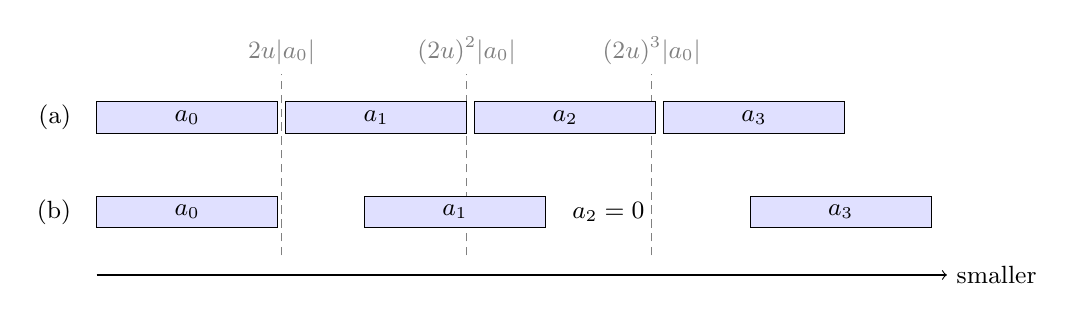
\begin{tikzpicture}[x=1cm, y=1cm]
  \foreach \i in {1,2,3} { \draw[densely dashed, gray] (2.35*\i, -1.75) -- (2.35*\i, 0.55); }
  \node[gray, font=\small, above] at (2.35, 0.55) {$2u|a_0|$};
  \node[gray, font=\small, above] at (4.70, 0.55) {$(2u)^2|a_0|$};
  \node[gray, font=\small, above] at (7.05, 0.55) {$(2u)^3|a_0|$};
  \node[left, font=\small] at (-0.2, 0) {(a)};
  \foreach \x/\l in {0/a_0, 2.4/a_1, 4.8/a_2, 7.2/a_3} {
    \draw[fill=blue!12] (\x, -0.2) rectangle ++(2.3, 0.4); \node[font=\small] at (\x+1.15, 0) {$\l$}; }
  \node[left, font=\small] at (-0.2, -1.2) {(b)};
  \draw[fill=blue!12] (0, -1.4) rectangle ++(2.3, 0.4); \node[font=\small] at (1.15, -1.2) {$a_0$};
  \draw[fill=blue!12] (3.4, -1.4) rectangle ++(2.3, 0.4); \node[font=\small] at (4.55, -1.2) {$a_1$};
  \node[font=\small] at (6.5, -1.2) {$a_2 = 0$};
  \draw[fill=blue!12] (8.3, -1.4) rectangle ++(2.3, 0.4); \node[font=\small] at (9.45, -1.2) {$a_3$};
  \draw[->] (0, -2.0) -- (10.8, -2.0) node[right, font=\small] {smaller};
\end{tikzpicture}
\caption{Two four-part expansions on the ladder. Each box is a part's $p$ significant bits, placed by its exponent.
(a)~Each part at most one ulp of the part above. (b)~A gap after $a_0$ and a zero part. A part may lie anywhere to the
right of its dashed line.}
\label{fig:ladder}
\end{figure}

\subsection{Error-free transformations}

\begin{samepage}
The algorithms are built from three operations that return a rounded result together with its exact
error~\cite{Dekker71,ORO05}:
\begin{itemize}
\item $\TwoSum(a, b)$ returns $s = \RN(a + b)$ and $e$ with $s + e = a + b$ exactly, using six operations;
\item $\FastTwoSum(a, b)$ returns the same $s$ and $e$ with three operations, but only when $|a| \ge |b|$;
\item $\TwoProd(a, b)$ returns $p = \RN(ab)$ and $e = ab - p$ exactly, using a product and one fused multiply-add.
\end{itemize}
\end{samepage}

\subsection{Multiplication by levels}

Write $a$ and $b$ with $a_0$ and $b_0$ of size about 1. The product $a_ib_j$ is then of size about $u^{i+j}$, and the
exact product is grouped by this \emph{order} $i + j$, as in the QD paper:
\[
ab = \underbrace{a_0b_0}_{\text{order } 0} + \underbrace{(a_0b_1 + a_1b_0)}_{\text{order } 1} +
\underbrace{(a_0b_2 + a_1b_1 + a_2b_0)}_{\text{order } 2} + \cdots
\]
Level $m$ collects everything of size about $u^m$. Each product of order below $n$ is split exactly by $\TwoProd$: its
rounded value goes to level $i + j$ and its error, about $u$ times smaller, to level $i + j + 1$. A value is added to a
level by $\TwoSum$, and the error of that addition is carried to the next level down, which we call a \emph{carry}. The
products of order $n$ are only needed to about $p$ bits, so they are summed with fused multiply-adds into level $n$.
The products of higher order are dropped. Figure~\ref{fig:levels} shows the scheme for $n = 4$, and
Algorithm~\ref{alg:mul} gives it in full.

\nopagebreak
\begin{figure}[H]
\centering
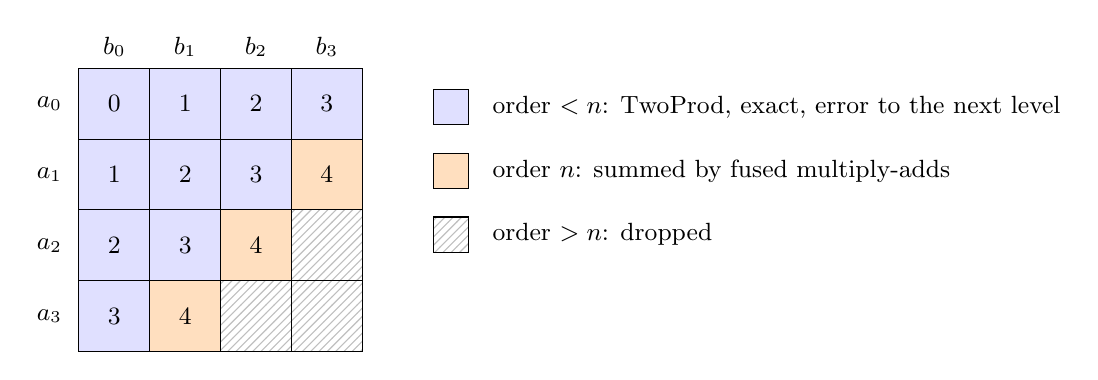
\begin{tikzpicture}[x=0.9cm, y=0.9cm]
  \foreach \i in {0,...,3} { \foreach \j in {0,...,3} {
    \pgfmathtruncatemacro{\o}{\i+\j}
    \ifnum\o<4 \fill[blue!12] (\j, -\i) rectangle ++(1, -1);
    \else\ifnum\o=4 \fill[orange!25] (\j, -\i) rectangle ++(1, -1);
    \else \fill[pattern=north east lines, pattern color=gray!50] (\j, -\i) rectangle ++(1, -1);
    \fi\fi
    \draw (\j, -\i) rectangle ++(1, -1);
    \ifnum\o<5 \node[font=\small] at (\j+0.5, -\i-0.5) {$\o$}; \fi } }
  \foreach \j in {0,...,3} { \node[font=\small] at (\j+0.5, 0.3) {$b_\j$}; }
  \foreach \i in {0,...,3} { \node[font=\small, anchor=east] at (-0.1, -\i-0.5) {$a_\i$}; }
  \begin{scope}[shift={(5, 0)}]
    \fill[blue!12] (0, -0.3) rectangle ++(0.5, -0.5); \draw (0, -0.3) rectangle ++(0.5, -0.5);
    \node[font=\small, anchor=west] at (0.7, -0.55) {order $< n$: $\TwoProd$, exact, error to the next level};
    \fill[orange!25] (0, -1.2) rectangle ++(0.5, -0.5); \draw (0, -1.2) rectangle ++(0.5, -0.5);
    \node[font=\small, anchor=west] at (0.7, -1.45) {order $n$: summed by fused multiply-adds};
    \fill[pattern=north east lines, pattern color=gray!50] (0, -2.1) rectangle ++(0.5, -0.5);
    \draw (0, -2.1) rectangle ++(0.5, -0.5);
    \node[font=\small, anchor=west] at (0.7, -2.35) {order $> n$: dropped};
  \end{scope}
\end{tikzpicture}
\caption{The partial products $a_ib_j$ of a four-part multiplication. Each cell shows the level its product goes
to, its order $i + j$. The five levels $0, \dots, 4$ are renormalized into four parts.}
\label{fig:levels}
\end{figure}

\begin{algorithm}[tp]
\caption{Multiplication of $n$-part expansions (MUL)}\label{alg:mul}
\begin{algorithmic}[1]
\Require $a = (a_0, \dots, a_{n-1})$, $b = (b_0, \dots, b_{n-1})$
\Ensure $x = (x_0, \dots, x_{n-1})$ with $\sum x_k \approx ab$
\For{$j = 0, \dots, n-1$} $(s_j, e_j) \gets \TwoProd(a_0, b_j)$ \Comment{levels $0, \dots, n-1$}
\EndFor
\State $s_n \gets \RN\bigl(\sum_{i=1}^{n-1} a_ib_{n-i}\bigr)$ by a chain of fused multiply-adds \Comment{order $n$}
\For{$j = 0, \dots, n-1$} $\dep(s, j+1, e_j)$
\EndFor
\For{$i = 1, \dots, n-1$ \textbf{and} $j = 0, \dots, n-1-i$}
  \State $(p, e) \gets \TwoProd(a_i, b_j)$; \ $\dep(s, i+j, p)$; \ $\dep(s, i+j+1, e)$
\EndFor
\State \Return $R_n(s_0, \dots, s_n)$ \Comment{Algorithm~\ref{alg:renorm}}
\Statex
\Statex \textbf{procedure} $\dep(s, l, t)$: add $t$ to level $l$ and carry its error down
\For{$m = l, \dots, n-1$} $(s_m, t) \gets \TwoSum(s_m, t)$
\EndFor
\State $s_n \gets \RN(s_n + t)$
\end{algorithmic}
\end{algorithm}

Addition works the same way: level $i$ starts as $\TwoSum(a_i, b_i)$, and each error is carried down. The product and
the sum of an expansion and a single floating-point number use the same scheme with fewer terms. The appendix lists
all four operations.

\subsection{Renormalization}

The levels overlap: level $m$ can hold bits that belong in level $m - 1$. The renormalization $R_n$
(Algorithm~\ref{alg:renorm}) turns $n + 1$ such terms into $n$ parts. Its first pass, VecSum~\cite{ORO05}, sweeps
from the smallest term to the largest with $\TwoSum$, which leaves the sum exact. Its second pass sweeps from the
largest term down and adds each term to an accumulator. When the addition is inexact, the rounded sum becomes the next
part and the error becomes the new accumulator, so the step \emph{emits} a part. When the addition is exact, the sum
stays in the accumulator.

\nopagebreak
\begin{algorithm}[H]
\caption{Renormalization $R_n$}\label{alg:renorm}
\begin{algorithmic}[1]
\Require terms $c_0, \dots, c_N$ with $N \le n$, in any order of magnitude
\Ensure $x = (x_0, \dots, x_{n-1})$
\State $s \gets c_N$
\For{$i = N-1, \dots, 0$} $(s, v_{i+1}) \gets \TwoSum(c_i, s)$ \Comment{VecSum}
\EndFor
\State $\acc \gets s$; \ $k \gets 0$; \ $x \gets (0, \dots, 0)$
\For{$j = 1, \dots, N$}
  \State $(t, e) \gets \TwoSum(\acc, v_j)$
  \If{$e \ne 0$ \textbf{and} $k < n-1$} $x_k \gets t$; \ $k \gets k + 1$; \ $\acc \gets e$ \Comment{emit}
  \Else{} $\acc \gets t$
  \EndIf
\EndFor
\State $x_k \gets \acc$
\end{algorithmic}
\end{algorithm}

The QD library uses $\FastTwoSum$ in both passes, and its authors note that the conditions under which this
renormalization works are not known~\cite{HLB01}. Here both passes use $\TwoSum$. In the second pass, $\FastTwoSum$
gives the same bits whenever $|\acc| \ge |v_j|$, which holds when the terms arrive in decreasing order. They need not:
when an operand has a gap, a level can be larger than the level above it, and then only $\TwoSum$ is exact.

\section{The results}

The error of every operation has the same leading term: $u^n$ times the exact result.

\begin{theorem}[Appendix, Theorem~\ref{thm:t3}]\label{thm:main}
Let $Z$ be the exact sum or product of two expansions on the ladder, or of an expansion on the ladder and a
floating-point number, and let $x$ be the computed $n$ parts. Then
\[
\Bigl|Z - \sum_k x_k\Bigr| \le u^n|Z| + \kappa_n\,u^{n+1}M,
\]
where $M = |a_0b_0|$ for a product and $M = |a_0| + |b_0|$ for a sum, and $\kappa_n$ is a constant that depends on
the operation and on $n$.
\end{theorem}

The first term is the bound of rounding $Z$ to a format with $np$ bits. The second term is a correction. For a product,
$M$ is within a factor of about $1 + 4u$ of $|Z|$, so the whole bound is relative. For a sum, $M$ is the size of the operands,
and after cancellation it can be much larger than $|Z|$, the form of QD's own addition bound~\cite{HLB01}. Table~\ref{tab:summary}
gives the bounds at $n = 8$ in binary64, and Table~\ref{tab:main} shows how the correction grows with $n$.

\nopagebreak
\begin{table}[H]
\centering
\begin{tabular}{lll}
\toprule
operation & error bound & input that reaches $u^8|Z|$ \\
\midrule
$a + b$ & $u^8|Z| + 2^{-33.0}u^8(|a_0| + |b_0|)$ & $(1, u, \dots, u^7) + (u^8, 0, \dots, 0)$ \\
$a + f$ & $u^8|Z| + 2^{-42.4}u^8(|a_0| + |f|)$ & $(1, u, \dots, u^7) + u^8$ \\
$a \times f$ & $u^8|Z| + 2^{-33.0}u^8|a_0f|$ & $f = 3$, Proposition~\ref{prop:sharp}(c) \\
$a \times b$ & $u^8|Z| + 2^{-15.1}u^8|a_0b_0|$ & $(1, u, \dots, u^6, 0) \times (1, 0, \dots, 0, u^7)$ \\
$a / b$ & $(1 + 2^{-25.5})\,u^8|Z|$ & $(1, 0, \dots, 0) / (-1, u, 0, \dots, 0)$ \\
$\sqrt a$ & $3.00004\,u^8|Z|$ & not known \\
\bottomrule
\end{tabular}
\caption{Proven error bounds at $n = 8$ parts in binary64, where $u^8 = 2^{-424}$, for expansions $a$ and $b$ on the
ladder and a floating-point number $f$. $Z$ is the exact result.}
\label{tab:summary}
\end{table}

\nopagebreak
\begin{table}[H]
\centering
\begin{tabular}{rccccc}
\toprule
$n$ & $u^n$ & $a + b$ & $a \times f$ & $a + f$ & $a \times b$ \\
\midrule
2 & $2^{-106}$ & $2^{-48.5}$ & $2^{-48.5}$ & $2^{-49.2}$ & $2^{-45.9}$ \\
4 & $2^{-212}$ & $2^{-43.8}$ & $2^{-43.8}$ & $2^{-46.6}$ & $2^{-37.3}$ \\
8 & $2^{-424}$ & $2^{-33.0}$ & $2^{-33.0}$ & $2^{-42.4}$ & $2^{-15.1}$ \\
12 & $2^{-636}$ & $2^{-19.6}$ & $2^{-19.6}$ & $2^{-38.4}$ & $2^{12.5}$ \\
\bottomrule
\end{tabular}
\caption{The second term of Theorem~\ref{thm:main} relative to the first, $\kappa_nu$, in binary64. The
multiplication's constant grows like $n(n!)^2$, and from eleven parts its second term is the larger one.}
\label{tab:main}
\end{table}

\begin{theorem}[Appendix, Theorems~\ref{thm:t6} and~\ref{thm:t7}]\label{thm:divsqrt}
For expansions on the ladder, long division with $n+1$ quotient terms errs by at most $(u^n + K_nu^{n+1})|a/b|$, with
$K_8u = 2^{-25.5}$ and $K_nu < 1$ up to $n = 13$ in binary64. The square root by four Newton steps errs by at most
$3.00004\,u^8\sqrt a$ at $n = 8$.
\end{theorem}

The bounds chain. At eight parts in binary64, a product of two expansions on the ladder is again on the ladder, and
so is a sum whose operands' leading parts have one sign (Corollary~\ref{cor:closure}), so the bounds apply at every
step of such a computation. A
subtraction of nearly equal values can leave the ladder, and a computation that cancels needs its own analysis, as
the division's remainders receive in the appendix.

\section{A worked example}\label{sec:example}

The bound $u^n|Z|$ is reached by simple inputs. Take $n = 3$ and multiply
\[
a = (1,\ u,\ 0), \qquad b = (1,\ 0,\ u^2).
\]
The exact product is $(1 + u)(1 + u^2) = 1 + u + u^2 + u^3$. Every partial product is a power of $u$ and exact, so
Algorithm~\ref{alg:mul} fills the levels with $1, u, u^2, u^3$, one power each. The renormalization then runs as
follows.
\begin{center}
\begin{tabular}{clll}
\toprule
step & $\TwoSum(\acc, v_j)$ & rounded sum and error & action \\
\midrule
1 & $1 + u$ & $1$, error $u$ & emit $x_0 = 1$ \\
2 & $u + u^2$ & $u$, error $u^2$ & emit $x_1 = u$ \\
3 & $u^2 + u^3$ & $u^2$, error $u^3$ & last part, keep $x_2 = u^2$ \\
\bottomrule
\end{tabular}
\end{center}
Each sum is a tie, exactly halfway between two floating-point numbers, and ties go to the even neighbor, which is the
power of $u$. The result is $(1, u, u^2)$, and the last error $u^3$ has nowhere to go. So
\[
\Bigl|Z - \sum_k x_k\Bigr| = u^3 = u^3|Z|\,(1 - O(u)).
\]
The loss is the algorithm's, not the format's: the three binary64 numbers $(1 + 2u,\ -(u - u^2),\ u^3)$ add up to $Z$
exactly. On this input, rounding ties away from zero returns that exact split.

The same construction works for every $n$, for each operation except the square root.

\begin{proposition}[Appendix, Proposition~\ref{prop:sharp}]\label{prop:worst}
The product of $(1, u, \dots, u^{n-2}, 0)$ and $(1, 0, \dots, 0, u^{n-1})$ for $n \ge 3$, the sum of $(1, u, \dots,
u^{n-1})$ and $(u^n, 0, \dots, 0)$, and the quotient of $(1, 0, \dots, 0)$ by $(-1, u, 0, \dots, 0)$ each return $\pm(1,
u, \dots, u^{n-1})$, and so err by $u^n|Z|$ up to a factor $1 - O(u)$. The product with a floating-point number has a
similar input.
\end{proposition}

Random inputs never come near this. At $n = 8$ in binary64, random operands give errors below $0.01\,u^8|Z|$ for every
operation in multidouble's tests. The error is about half an ulp of the result's last part, and a random result's last
part is far smaller than the ladder allows. Multidouble's octo-double~\cite{md} returns exactly $\pm(1, u, \dots, u^7)$
on the product, sum and quotient inputs.

\section{Why the bounds hold}

\paragraph{The renormalization loses only at its last step.} Each step of the second pass either keeps the sum exactly
in the accumulator or emits a part and carries the exact error. So nothing is lost until all $n$ parts are filled. Only
the last step can lose its error, and only when every step before it emitted a part, as in the example above. That
error is the last of a chain of $n$ rounding errors, each at most $u$ times the one before, which gives the factor
$u^n$.

\begin{theorem}[Appendix, Theorem~\ref{thm:t1}]\label{thm:renorm}
For $n$ or fewer terms in any order, the renormalization is exact. For $n + 1$ terms it loses at most
$u^n|v_0| + \sum_{j=1}^{n}u^{n+1-j}|v_j|$, where $v$ is VecSum's output, and this is attained.
\end{theorem}

Earlier analyses of renormalization assumed that the terms arrive in decreasing order and do not
overlap~\cite{JMMP16,BJMP17,FMP19}. Theorem~\ref{thm:renorm} needs neither, because $\TwoSum$ is exact for terms in any
order. With $\FastTwoSum$ alone, the same pass can drop terms when an operand has a gap: at $n = 8$, terms of
relative size $2^{-325}$. The same failure has been seen elsewhere. Kouya~\cite{Kouya26} gives an input whose VecSum
output is out of order, so that a following $\FastTwoSum$ chain drops a term. The Universal library found its
quad-double addition losing accuracy when QD's renormalization received overlapping terms~\cite{universal}.

\paragraph{The levels stay small.} The second term of Theorem~\ref{thm:main} comes from bounding each level. Every
carry out of a level is at most $u$ times what the level holds, so level $m$ stays of size about $u^m|a_0b_0|$, up to
a factor that counts the $\TwoSum$s it went through, $m(m+1)$ at level $m$ of the multiplication. The carries feed back
into the levels' sizes, which gives a recursion for the bounds (Lemma~\ref{lem:l} and Theorem~\ref{thm:t2}). The
dropped products of order above $n$ are bounded directly. With level $m$ at most $L_mu^mM$,
Theorem~\ref{thm:renorm} gives Theorem~\ref{thm:main}. The division and the square root follow by carrying a bound on
each part through every step (Lemma~\ref{lem:g}).

\section{Consequences and limits}

\begin{itemize}
\item \textbf{Testing.} A library tested only on random inputs is not tested against $u^n$. At $n = 8$, random
  errors stay below $0.01\,u^8|Z|$. The inputs of Proposition~\ref{prop:worst} reach the bound exactly and make sharp tests.
\item \textbf{Renormalization.} The second pass should use $\TwoSum$, or $\FastTwoSum$ after a test that
  $|\acc| \ge |v_j|$, which gives the same bits.
\item \textbf{Many parts.} The multiplication's correction grows like $n(n!)^2$. Beyond ten parts in binary64 the
  bound still holds, but it is no longer close to $u^n$.
\item \textbf{Underflow.} The hypotheses exclude underflow in any intermediate value, not only in the operands. A part
  far below the one above it can make a product of two small parts underflow.
\item \textbf{Open questions.} The second-order constants come from triangle inequalities and are not claimed to be
  tight. Whether the square root's constant 3 is reached is open. Sums of products accumulated in levels, as
  dot-product kernels do, are not covered.
\end{itemize}

\section{Computations}

The constants were evaluated in exact rational arithmetic (\texttt{constants.py}, \texttt{div\_consts.py},
\texttt{sqrt\_consts.py}). A reviewer who had not seen the checks recomputed them from the definitions with separate
code, and the values agree to the digits given.

Every statement was also tested by an independent emulator, written from multidouble's source without access to the
proofs. It reproduces multidouble's octo-double bit for bit on 10,000 inputs of each operation. It ran the algorithms
in exact arithmetic at precisions 5 to 10 with 5 to 8 parts, over exhaustive families of ladders, gaps, zero parts,
cancelling pairs and shuffled orders, and at random and by hill climbing, about 37 million renormalizations in all,
and at $p = 53$. No statement failed. The bounds of Theorem~\ref{thm:renorm} and Proposition~\ref{prop:worst} were
reached with ratio 1, and each check fired on a halved bound or a deliberately broken algorithm. The example of
Section~\ref{sec:example} was run on the same emulator (\texttt{example\_n3.py}).

Multidouble's own tests check the bound of Theorem~\ref{thm:main} against exact arithmetic on every random input that
meets the hypotheses, and pin the inputs of Proposition~\ref{prop:worst}.

\section*{How this work was done}

Nathan Moinvaziri posed the problem and directed the work. Claude, an AI model made by Anthropic, drafted the
statements and proofs. Two further Claude instances checked them independently: one refereed the proofs and the prior
work, and the other tested every statement in exact arithmetic without reading the proofs.

\clearpage
\appendix
\section{Setting}

\begin{assumption}\label{as:fp}
(A1) $\F$ is the set of binary floating-point numbers of precision $p \ge 3$, with $u = 2^{-p}$. Addition,
multiplication, division, square root and the fused multiply-add are correctly rounded to nearest with ties to even
($\RN$). (A2) No underflow or overflow occurs: every operation returns
what it would return in the same format with an unbounded exponent range.
\end{assumption}

Write $\us = u/(1+u)$. Under (A2), for every real $z$,
\begin{gather}
|\RN(z) - z| \le \us |z|, \qquad |\RN(z) - z| \le u\,|\RN(z)|, \label{eq:rn} \\
\frac{|z|}{1+u} \le |\RN(z)| \le (1+u)|z|. \nonumber
\end{gather}
The second inequality follows from the first, since $|z| \le |\RN(z)| + |\RN(z) - z|$ and $\us/(1-\us) = u$. The
number of parts is $n \ge 2$, and we write (A3) for the condition $(n^2+n)u < 1$, assumed only where it is named. A sum
whose upper limit is below its lower one is zero.

Assumption (A2) concerns each run, not only the operands' values. For binary64 it holds when no result overflows,
every exact value that the run rounds is zero, at least $2^{-1022}$ in magnitude, or a multiple of $2^{-1074}$ (and
then representable), and every $\TwoProd(a, b)$ has $e_a + e_b \ge -1022 + 52$, the classical condition for its
error to be representable, with $e_x$ the exponent of $x$. A part far below the one above it can make a product of
two small parts underflow even when the operands are far above $2^{-1022}$; the bounds here do not cover such runs.

\begin{definition}\label{def:h}
For $1 \le \theta \le 1/(4u)$, an $n$-part $a = (a_0, \dots, a_{n-1}) \in \F^n$ satisfies $H(\theta)$ when $|a_i| \le
\rho^i |a_0|$ for $1 \le i \le n-1$, where $\rho = \theta u$ here and throughout, so that $\rho \le 1/4$.
\end{definition}

Since $\ulp(x) \le 2u|x|$, an ulp-nonoverlapping expansion \cite{MPT16,BJMP17} ($|a_{i+1}| \le \ulp(a_i)$, with
$\ulp(0) = 0$) satisfies $H(2)$, and one with $|a_{i+1}| \le \frac12\ulp(a_i)$ (B-nonoverlapping in \cite{JMMP16})
satisfies $H(1)$. If $a_0 = 0$, $H(\theta)$ forces $a = 0$; when the scale $M$ below is zero the operands are zero and
the results are exact, so we take $M > 0$. The hypothesis allows a part far
below the one above it, and zero parts between nonzero ones, as long as the ladder relative to $a_0$ holds. If $a$
satisfies $H(\theta)$, then
\begin{equation}\label{eq:a0}
|a| \ge |a_0|\Bigl(1 - \sum_{i \ge 1}\rho^i\Bigr) = \frac{1-2\rho}{1-\rho}\,|a_0|, \qquad |a| = \Bigl|\sum_i a_i\Bigr|,
\end{equation}
and so its parts are bounded by its value:
\begin{equation}\label{eq:abar}
|a_i| \le \bar a_i\,|a|, \qquad \bar a_i = \rho^i\,\frac{1-\rho}{1-2\rho}.
\end{equation}

\section{The algorithms}

$\TwoSum(a, b)$ returns $s = \RN(a+b)$ and $e = \RN(\RN(a - \RN(s - b')) + \RN(b - b'))$ with $b' = \RN(s - a)$;
$\FastTwoSum(a, b)$ returns $s = \RN(a+b)$ and $e = \RN(b - \RN(s - a))$; $\TwoProd(a, b)$ returns $p = \RN(ab)$ and $e
= \RN(ab - p)$, by one FMA.

On levels $s_0, \dots, s_n$, $\dep(s, l, t)$ sets $e \gets t$, then for $m = l, \dots, n-1$ performs $(s_m, e) \gets
\TwoSum(s_m, e)$, and finally $s_n \gets \RN(s_n + e)$. The error moved from level $m$ to level $m+1$ is a \emph{carry}.

\parhead{VecSum} For $c = (c_0, \dots, c_{N-1})$: $s \gets c_{N-1}$; for $i = N-2, \dots, 0$, $(s, v_{i+1}) \gets
\TwoSum(c_i, s)$; then $v_0 \gets s$. We write $s_i$ for the value of $s$ after the step with index $i$, so $s_{N-1} =
c_{N-1}$, $s_i = \RN(c_i + s_{i+1})$ and $v_0 = s_0$.

\parhead{Renormalization $\Ren_n$} For $c \in \F^N$ with $N \le n+1$, let $v = \mathrm{VecSum}(c)$, $k \gets 0$, $\acc
\gets v_0$ and $x \gets 0 \in \F^n$. Step $j$, for $j = 1, \dots, N-1$, forms $(t, e) \gets \TwoSum(\acc, v_j)$. If $k <
n-1$ and $e \ne 0$, the step \emph{emits}: $x_k \gets t$, $k \gets k+1$, $\acc \gets e$. Otherwise $\acc \gets t$.
Finally $x_k \gets \acc$. We write $\acc_j$ for $\acc$ after step $j$, and $\acc_0 = v_0$.

\parhead{Operations} For $n$-part $a$ and $b$, and $b \in \F$ where noted:
\begin{itemize}
\item ADD: $(s_i, t_i) \gets \TwoSum(a_i, b_i)$ for $i < n$; $s_n \gets t_{n-1}$; $\dep(s, l, t_{l-1})$ for $l = 1,
\dots, n-1$; return $\Ren_n(s)$.
\item ADDF ($b \in \F$): $e \gets b$; $(s_i, e) \gets \TwoSum(a_i, e)$ for $i = 0, \dots, n-1$; $s_n \gets e$; return
$\Ren_n(s)$.
\item MULF ($b \in \F$): $(s_i, e_i) \gets \TwoProd(a_i, b)$ for $i < n$; $s_n \gets e_{n-1}$; $\dep(s, l, e_{l-1})$ for
$l = 1, \dots, n-1$; return $\Ren_n(s)$.
\item MUL: (1) $(s_j, e_{0j}) \gets \TwoProd(a_0, b_j)$ for $j < n$. (2) $s_n \gets \RN(a_1 b_{n-1})$, then $s_n \gets
\RN(a_i b_{n-i} + s_n)$ for $i = 2, \dots, n-1$. (3) $\dep(s, l, e_{0,l-1})$ for $l = 1, \dots, n$. (4) For
$i = 1, \dots, n-1$ and $j = 0, \dots, n-1-i$: $(p_{ij}, e_{ij}) \gets \TwoProd(a_i, b_j)$, $\dep(s, i+j, p_{ij})$,
$\dep(s, i+j+1, e_{ij})$. (5) Return $\Ren_n(s)$.
\end{itemize}
At $n = 8$ and $p = 53$ these are the octo-double algorithms of multidouble~\cite{md}. Its scalar type takes $\FastTwoSum$
instead of $\TwoSum$ in the second pass when $|\acc| \ge |v_j|$, which by Lemma~\ref{lem:facts}(b) gives the same bits.

\begin{lemma}[standard]\label{lem:facts}
Under Assumption~\ref{as:fp}: (a) $\TwoSum(a, b) = (s, e)$ satisfies $s + e = a + b$ and $|e| \le \min(|a|, |b|, \us|a+b|)$;
$e = 0$ if and only if $a + b \in \F$. (b) If $|a| \ge |b|$, $\FastTwoSum(a, b)$ returns the $s$ and $e$ of
$\TwoSum(a,b)$, up to the sign of a zero $e$. (c) $\TwoProd(a, b) = (p, e)$ satisfies $p + e = ab$, $|e| \le \us|ab|$
and $|p| \le (1+u)|ab|$.
\end{lemma}

\begin{proof}
(a) Exactness is M{\o}ller's and Knuth's~\cite{Moller65,Knuth97}. Since $a$ and $b$ are in $\F$ and lie at distances $|b|$ and $|a|$ from $a+b$, the nearest
element $s$ is at least as close: $|e| = |a + b - s| \le \min(|a|, |b|)$. The third bound is \eqref{eq:rn}. (b) With
$|a| \ge |b|$ the exponent of $a$ is at least that of $b$, so $\FastTwoSum$ is exact \cite{Dekker71}, and both errors
equal $a + b - s$. (c) Under (A2), $ab - p \in \F$, so the FMA returns it exactly; the bounds are \eqref{eq:rn}.
\end{proof}

\section{Renormalization in any order}

\begin{theorem}\label{thm:t1}
Under Assumption~\ref{as:fp}, let $c \in \F^{n+1}$, in any order of magnitudes, $v = \mathrm{VecSum}(c)$, $x = \Ren_n(c)$, $S =
\sum_m c_m$ and $E = S - \sum_k x_k$.
\begin{enumerate}
\item[(a)] $\sum_j v_j = S$. If $\Ren_n$ is given $N \le n$ terms, $E = 0$. With $N = n+1$, $E \ne 0$ only if each of the
steps $1, \dots, n-1$ emitted. Then $\acc_j$ is the error of the $\TwoSum$ of step $j$ for $1 \le j \le n-1$, and $E =
\acc_{n-1} + v_n - x_{n-1}$ is the error of the $\TwoSum$ of step $n$.
\item[(b)] $|E| \le \min_{0 \le k \le n} B_k$, where
\[
B_k = \us^{\,n-k}|v_k| + \sum_{j=k+1}^{n} \us^{\,n+1-j}|v_j|.
\]
\item[(c)] For $c = (1, u, u^2, \dots, u^n)$, $v = c$ and $|E| = B_0 = u^n$.
\item[(d)] With $\sigma_l = \sum_{m \ge l}|c_m|$: $|v_0| \le (1+u)^n\sigma_0$, and $|v_j| \le \min\bigl(|c_{j-1}|,\
\us(1+u)^{n-j}\sigma_{j-1}\bigr)$ for $1 \le j \le n$.
\item[(e)] If $|c_m| \le L_m u^m M$ for $0 \le m \le n$, with $M > 0$, then
\begin{gather*}
|E| \le u^n|S| + \frac{2(1+u)^{n-1}}{1-u}\,\Lambda\,u^{n+1}M, \\
\Lambda = \sum_{m=0}^{n} L_m.
\end{gather*}
\end{enumerate}
\end{theorem}

\begin{proof}
(a) Each $\TwoSum$ of VecSum is exact, so $\sum_j v_j = S$. In the second pass every step has $\acc + v_j = t + e$
exactly. An emitting step stores $t$ and carries $e$. A step that does not emit and has $e = 0$ sets $\acc = \acc +
v_j$. In both cases $\sum_{i<k} x_i + \acc + \sum_{i>j} v_i$ keeps the value $S$. Only a step with $k = n-1$ and $e \ne
0$ changes it, by $-e$, and the final $x_k \gets \acc$ is exact. Each step raises $k$ by at most one, so before step $j$,
$k \le j - 1$. A step with $k = n-1$ therefore has $j \ge n$. With $N \le n$ there are at most $n-1$ steps, and $E =
0$. With $N = n+1$ only step $n$ can lose its error, and only when $k = n-1$ before it, that is, when each of the steps
$1, \dots, n-1$ emitted. Then $\acc_j$ is the error of step $j$ for $j \le n-1$, step $n$ sets $x_{n-1} = t$, and $E$
is its error.

(b) If $E = 0$ there is nothing to prove. Otherwise (a) applies; set $\acc_n = E$. For $1 \le j \le n$, $\acc_j$ is the
error of $\TwoSum(\acc_{j-1}, v_j)$, so by Lemma~\ref{lem:facts}(a)
\begin{gather*}
|\acc_j| \le \us|\acc_{j-1} + v_j| \le \us|\acc_{j-1}| + \us|v_j|, \\
|\acc_j| \le |v_j|.
\end{gather*}
Iterating the first inequality from $j = k+1$ to $n$ gives $|E| \le \us^{\,n-k}|\acc_k| + \sum_{j=k+1}^n
\us^{\,n+1-j}|v_j|$, and $|\acc_k| \le |v_k|$ (for $k \ge 1$ by the second inequality, for $k = 0$ by definition).

(c) For $i \ge 0$, $u^i + u^{i+1} = u^i(1 + 2^{-p})$ is the midpoint of $u^i$ and its successor $u^i(1 + 2^{1-p})$, so
$\RN$ returns $u^i$, whose significand is even, with error $u^{i+1}$. Hence VecSum returns $v = c$. In the second pass,
step $j$ computes $\TwoSum(u^{j-1}, u^j) = (u^{j-1}, u^j)$, so steps $1, \dots, n-1$ emit and step $n$ loses $E =
u^n$. Finally $\sum_{i=1}^n u\,(1+u)^{-i} = 1 - (1+u)^{-n}$ gives
\begin{align*}
B_0 &= \frac{u^n}{(1+u)^n} + \sum_{j=1}^{n}\frac{u^{n+1-j}}{(1+u)^{n+1-j}}\,u^j \\
&= u^n\Bigl((1+u)^{-n} + 1 - (1+u)^{-n}\Bigr) = u^n.
\end{align*}

(d) By induction from $s_n = c_n$, $|s_i| = |\RN(c_i + s_{i+1})| \le (1+u)\bigl(|c_i| + (1+u)^{n-i-1}\sigma_{i+1}\bigr)
\le (1+u)^{n-i}\sigma_i$; in particular $|v_0| = |s_0| \le (1+u)^n\sigma_0$. For $j \ge 1$, $v_j$ is the error of
$\TwoSum(c_{j-1}, s_j)$, so $|v_j| \le |c_{j-1}|$ and $|v_j| \le \us(|c_{j-1}| + |s_j|) \le \us(1+u)^{n-j}\sigma_{j-1}$.

(e) Take $k = 0$ in (b) and $\us \le u$. By (d), and $\sigma_l \le M\sum_{m \ge l} L_m u^m$,
\begin{align*}
&\sum_{j=1}^n u^{n+1-j}|v_j| \\
&\quad\le u^{n+1}M\sum_{j=1}^n (1+u)^{n-j}\sum_{m=j-1}^{n} L_m u^{m-j+1} \\
&\quad\le u^{n+1}M(1+u)^{n-1}\sum_{m=0}^n L_m \sum_{i \ge 0} u^i = \frac{(1+u)^{n-1}}{1-u}\Lambda u^{n+1}M,
\end{align*}
since for fixed $m$ the exponents $m - j + 1$, $1 \le j \le \min(m+1, n)$, are distinct and nonnegative. Likewise,
using $(m+1)u^m \le 1$ for $u \le 1/2$,
\begin{align*}
|v_0| &\le |S| + \sum_{j=1}^n |v_j| \\
&\le |S| + u(1+u)^{n-1}M\sum_{m=0}^n (m+1)L_m u^m \\
&\le |S| + u(1+u)^{n-1}\Lambda M,
\end{align*}
so $u^n|v_0| \le u^n|S| + (1+u)^{n-1}\Lambda u^{n+1}M$. Adding the two bounds gives (e).
\end{proof}

\begin{remark}
With \eqref{eq:rn}, part (a) gives $|E| \le \frac12\ulp(x_{n-1})$. Part (b) needs no hypothesis on the order of the
terms. Of the earlier analyses, \cite{JMMP16,BJMP17} prove exactness and nonoverlap of the renormalization for terms
that overlap by at most $p-2$ digits, and \cite{FMP19} (Thm.~3) bounds the error of a truncation of ordered terms. By
(c), the leading constant 1 in (b) and (e) is attained. With $N = n$ terms, as in
\texttt{OD::new}, the renormalization is exact.
\end{remark}

\section{The levels}

\begin{lemma}\label{lem:l}
Under Assumption~\ref{as:fp}, let levels $s_0, \dots, s_n$ start at zero and be changed only by (i) assignments $s_m \gets y$ to
a zero level, (ii) calls $\dep(s, l, t)$, and (iii) roundings $s_n \gets \RN(s_n + y)$ for real $y$ that are not the
last step of a dep. Let $A_m$ be the sum of $|y|$ over (i) at level $m$, of $|t|$ over the calls with $l = m$, and, for
$m = n$, of $|y|$ over (iii). Let $T_m$ be the number of $\TwoSum$s at level $m < n$, $Q$ the number of roundings at
level $n$ (those of (iii) and the last steps of the deps), and assume $T_m u < 1$ and $Qu < 1$. Let $D_0 = A_0$ and, for
$0 \le m \le n-1$,
\begin{gather*}
C_m = \frac{T_m u\,D_m}{1 - T_m u}, \qquad D_{m+1} = A_{m+1} + C_m, \\
X_m = \frac{D_m}{1 - T_m u}\ (m < n), \qquad X_n = \frac{D_n}{1 - Qu}, \qquad R = QuX_n.
\end{gather*}
Then: (a) at every moment $|s_m| \le X_m$; (b) the carries out of
level $m$ have absolute sum at most $C_m$; (c) at the end, $\sum_m s_m = Y - \sum r$, where $Y$ is the sum (with signs)
of the $y$ of (i) and (iii) and the $t$ of (ii), and the rounding errors $r$ at level $n$ satisfy $\sum|r| \le R$.
\end{lemma}

\begin{proof}
Fix $m < n$. A $\TwoSum$ at level $m$ replaces $s_m$ by $s_m + y - e$, where $y$ is a deposited $t$ or a carry from
level $m-1$ and $e$ is the carry out. So at every moment $s_m$ equals the signed sum of everything put into level $m$
so far minus the carries out so far. Let $\hat D_m$ be the total of $|\cdot|$ over everything put into level $m$
during the run, and $\hat C_m$ the total of the carries out. The value $s_m + y$ that a $\TwoSum$ rounds is of the same
form, so $|s_m + y| \le \hat D_m + \hat C_m$, and Lemma~\ref{lem:facts}(a) bounds its carry by $u(\hat D_m + \hat
C_m)$. Summing over the $T_m$ $\TwoSum$s, $\hat C_m \le T_m u(\hat D_m + \hat C_m)$, that is, $\hat C_m \le T_m u \hat
D_m/(1 - T_m u)$, and $|s_m| \le \hat D_m + \hat C_m \le \hat D_m/(1 - T_m u)$ at every moment. Level 0 receives no
carries, so $\hat D_0 = A_0 = D_0$. Each carry out of level $m$ goes into level $m+1$ (for $m = n-1$, by the last step
of its dep), so $\hat D_{m+1} \le A_{m+1} + \hat C_m$. By induction on $m$, $\hat D_m \le D_m$ and $\hat C_m \le C_m$,
which gives (a) and (b) below level $n$. A dep started at level $n$ is a single rounding there; it is counted in $Q$,
and its input in $A_n$.

At level $n$, a rounding $s_n \gets \RN(s_n + y)$, with $y$ from (iii) or a carry, has $|s_n + y| \le \hat D_n + \hat
R$, where $\hat D_n \le A_n + C_{n-1} = D_n$ is the total put into level $n$ and $\hat R$ the total of the rounding
errors. By \eqref{eq:rn} each error is at most $u(\hat D_n + \hat R)$, so $\hat R \le Q u \hat D_n/(1 - Qu) \le R$ and
$|s_n| \le \hat D_n + \hat R \le D_n/(1-Qu)$. For (c): an assignment or a deposit adds $y$ or $t$ to $\sum_m s_m$; a
$\TwoSum$ moves its carry from one level to the next without changing the sum; a rounding at level $n$ adds $y - r$ (a
carry $y$ having already been counted where it entered).
\end{proof}

\section{Operations from part bounds}

\begin{lemma}\label{lem:o}
Under Assumption~\ref{as:fp}, for $c \in \F^{n+1}$, $v = \mathrm{VecSum}(c)$, $x = \Ren_n(c)$, $S = \sum_m c_m$ and $W_k =
\sum_{j=k+1}^{n}|v_j|$,
\begin{gather*}
\frac{|S| - W_1}{1+u} \le |x_0| \le (1+u)(|S| + W_1), \\
|x_i| \le (1+u)(u|x_{i-1}| + W_i) \quad (1 \le i \le n-1).
\end{gather*}
\end{lemma}

\begin{proof}
Let the pass emit $q$ times, at steps $j_0 < \dots < j_{q-1}$, with errors $\varepsilon_0, \dots, \varepsilon_{q-1}$. By
\eqref{eq:rn}, $|\varepsilon_i| \le u|x_i|$. Each emission happens at a later step than the one before, so $j_{i-1}
\ge i$. Between two emissions every step has $e = 0$ and adds exactly, except a final lossy step $n$ (Theorem
\ref{thm:t1}(a)). So for $1 \le i \le q - 1$, $x_i = \RN(\varepsilon_{i-1} + \sum_{j_{i-1} < j \le j_i} v_j)$, and $x_q$
is $\varepsilon_{q-1} + \sum_{j > j_{q-1}} v_j$, exactly or rounded once; the parts after $x_q$ are zero. With
\eqref{eq:rn}, $|x_i| \le (1+u)(u|x_{i-1}| + W_{j_{i-1}}) \le (1+u)(u|x_{i-1}| + W_i)$. If $q = 0$, nothing is lost
($n \ge 2$), and $x_0 = S$. Otherwise $x_0 = \RN(\sum_{j \le j_0} v_j)$ with $\bigl||\sum_{j \le j_0} v_j| - |S|\bigr|
\le W_{j_0} \le W_1$.
\end{proof}

\begin{lemma}\label{lem:g}
Under Assumption~\ref{as:fp} and (A3), let the operands' parts satisfy $|a_i| \le \alpha_i$ and $|b_j| \le \beta_j$
($\beta_0 \ge |b|$ for ADDF and MULF), let $Z$ be the exact result and $\bar Z \ge |Z|$, and let $P_m =
\sum_{i+j=m}\alpha_i\beta_j$ over the parts' indices $0 \le i, j < n$, $\lambda_m \ge |a_m + b_m|$ for ADD and
$\lambda_m = \alpha_m\beta_0$ for MULF, with $P_{-1} = \lambda_{-1} = 0$, and $m < n$ in the row of $A_m$:
\[
\begin{tabular}{@{}lll@{}}
\toprule
& MUL & ADD, MULF \\
\midrule
$A_m$ & $(1+u)P_m + uP_{m-1}$ & $(1+u)\lambda_m + u\lambda_{m-1}$ \\
$A_n$ & $P_n + uP_{n-1}$ & $u\lambda_{n-1}$ \\
$T_m$ & $m(m+1)$ & $m$ \\
$Q$ & $n^2 + n - 1$ & $n-1$ \\
$\Delta$ & $\sum_{m > n}P_m$ & $0$ \\
\bottomrule
\end{tabular}
\]
Let $X_m$ and $R$ be those of Lemma~\ref{lem:l}. For
ADDF, with $\lambda_0 \ge |a_0 + b|$, let $\epsilon_0 = u\lambda_0$, $\epsilon_m = u(\alpha_m + \epsilon_{m-1})$, $X_0
= (1+u)\lambda_0$, $X_m = (1+u)(\alpha_m + \epsilon_{m-1})$ for $1 \le m < n$, $X_n = \epsilon_{n-1}$ and $R = \Delta =
0$. With $\sigma_l = \sum_{m \ge l}X_m$, $V_j = \min(X_{j-1}, \us(1+u)^{n-j}\sigma_{j-1})$ and $W_k = \sum_{j > k}V_j$:
\begin{enumerate}
\item[(a)] $|Z - \sum_k x_k| \le u^n\bar Z + (1+u^n)(R+\Delta) + \sum_{j=1}^n (u^n + u^{n+1-j})V_j$;
\item[(b)] $|x_0| \le (1+u)(\bar Z + R + \Delta + W_1)$, and $|x_i| \le (1+u)(u|x_{i-1}| + W_i)$ for $1 \le i < n$;
\item[(c)] the levels satisfy $|s_m| \le X_m$ at every moment, and their final values $c$ satisfy $|Z - \sum_m c_m| \le
  R + \Delta$; for MUL, ADD and MULF the level array has exactly $T_m$ $\TwoSum$s at level $m < n$ and $Q$ roundings at
  level $n$.
\end{enumerate}
\end{lemma}

\begin{proof}
MUL, ADD and MULF are programs of the form of Lemma~\ref{lem:l}.

\emph{MUL.} Level 0 holds $\RN(a_0b_0)$, at most $(1+u)P_0$. For $1 \le m \le n-1$, level $m$ receives the products
$p_{ij}$ with $i + j = m$, by assignment for $i = 0$ and by dep otherwise, each at most $(1+u)\alpha_i\beta_j$, and the
errors $e_{ij}$ with $i + j = m - 1$, each at most $u\alpha_i\beta_j$ by Lemma~\ref{lem:facts}(c). Level $n$ receives
the exact products $a_ib_{n-i}$ of step (2) and the errors $e_{ij}$ with $i + j = n-1$. So the inputs of level $m$
total at most $A_m$ for every $m$. A dep started at level $l \le n-1$ performs one $\TwoSum$ at each level $l, \dots,
n-1$ and one rounding at level $n$. The deps started at a level $l \le m$ are $m$ of step (3), $m(m+1)/2$ products and
$m(m-1)/2$ errors of step (4), so $T_m = m + m^2$. The roundings at level $n$ are the $n-1$ of step (2) and one per
dep, $n + n(n-1)$ of them, so $Q = n^2 + n - 1$. Steps (1), (3) and (4) put in $p_{ij} + e_{ij} = a_ib_j$ for every $i
+ j \le n-1$ and step (2) the products of order $n$, so by Lemma~\ref{lem:l}(c) and the exactness of $\TwoSum$ and
$\TwoProd$ the final levels sum to $\sum_{i+j \le n} a_ib_j - \sum r$, and the dropped products total at most $\Delta$.

\emph{ADD and MULF.} Level $m < n$ holds $\RN(a_m + b_m)$ or $\RN(a_m b)$, at most $(1+u)\lambda_m$, and for $m \ge 1$
receives $t_{m-1}$ or $e_{m-1}$, at most $u\lambda_{m-1}$; level $n$ holds $t_{n-1}$ or $e_{n-1}$. The deps start at $l
= 1, \dots, n-1$, so $T_m = m$ and $Q = n-1$, and the final levels sum to $Z - \sum r$.

For these three, Lemma~\ref{lem:l} gives $|s_m| \le X_m$ at every moment and $\sum|r| \le R$, so $S = \sum_m c_m$ has
$F = |Z - S| \le R + \Delta$.

\emph{ADDF.} Here $s_m = \RN(a_m + e_{m-1})$ with $e_{-1} = b$, $e_m$ its error, and $s_n = e_{n-1}$; every operation
is exact, so the levels sum to $a + b$ and $F = 0$. By Lemma~\ref{lem:facts}(a), $|e_m| \le u(|a_m| + |e_{m-1}|)$, so
$|e_m| \le \epsilon_m$ and $|s_m| \le X_m$. This is (c).

Theorem~\ref{thm:t1}(d) gives $|v_j| \le V_j$ for $j \ge 1$, and Theorem~\ref{thm:t1}(b) with $k = 0$ and $|v_0| \le |S|
+ \sum_{j \ge 1}|v_j| \le \bar Z + F + \sum_{j \ge 1}V_j$ gives (a) after adding $F$. Lemma~\ref{lem:o} with $|S| \le
\bar Z + F$ gives (b).
\end{proof}

We write $(\epsilon, \pi') = G_{\rm OP}(\alpha, \beta;\ \bar Z)$ for the error bound (a) and the part bounds (b) that
Lemma~\ref{lem:g} gives for the operation OP, taking $\lambda_m = \alpha_m + \beta_m$ for ADD and $\lambda_0 = \alpha_0
+ \beta_0$ for ADDF, and $G_{\rm OP}(\alpha, \beta;\ \bar Z, \lambda)$ when $\lambda$ is given. A one-part operand $f$
has part bounds $(|f|, 0, \dots, 0)$, and
as an operand $|c|$ stands for the magnitudes of the parts of a constant expansion $c$. The bounds are homogeneous of
degree one in the operands' part bounds, $\lambda$ and $\bar Z$ together, so an operation on operands scaled exactly by
powers of two has the scaled bounds.

\section{Error bounds for the operations}\label{sec:bounds}

\begin{theorem}\label{thm:t2}
Under Assumption~\ref{as:fp} and (A3), let the $n$-part operands
satisfy $H(\theta)$ ($b \in \F$ arbitrary for ADDF and MULF). For MUL, ADD and MULF let $M$, $\hat A_m$, $T_m$ and $Q$ be
\begin{center}
\setlength{\tabcolsep}{5pt}
{\footnotesize\setlength{\tabcolsep}{2.5pt}\begin{tabular}{lccc}
\toprule
& MUL & ADD & MULF \\
\midrule
$M$ & $|a_0 b_0|$ & $|a_0| + |b_0|$ & $|a_0 b|$ \\
$\hat A_0$ & $1+u$ & $1+u$ & $1+u$ \\
$\hat A_m$, $0 < m < n$ & $(1+u)(m+1) + m/\theta$ & $1 + u + 1/\theta$ & $1 + u + 1/\theta$ \\
$\hat A_n$ & $n-1 + n/\theta$ & $1/\theta$ & $1/\theta$ \\
$T_m$ & $m(m+1)$ & $m$ & $m$ \\
$Q$ & $n^2 + n - 1$ & $n-1$ & $n-1$ \\
\bottomrule
\end{tabular}}
\end{center}
let $\Delta_n = \sum_{k=n+1}^{2n-2}(2n-1-k)\theta^k u^{k-n-1}$ for MUL and $\Delta_n = 0$ for ADD and MULF,
and let $d_0 = \hat A_0$ and, for $0 \le m \le n-1$,
\begin{gather*}
\gamma_m = \frac{T_m d_m}{\theta(1 - T_m u)}, \quad L_m = \frac{\theta^m d_m}{1 - T_m u}, \\
d_{m+1} = \hat A_{m+1} + \gamma_m,
\end{gather*}
and let $L_n = \theta^n d_n/(1 - Qu)$ and $R_n = QL_n$.
Then the level array of MUL, ADD and MULF has exactly $T_m$ $\TwoSum$s at level $m$ and $Q$ roundings at level $n$,
(a) $|s_m| \le L_m u^m M$ at every moment, for $0 \le m \le n$, and (b) the final levels $c$ satisfy $|Z - \sum_m c_m|
\le (R_n + \Delta_n)u^{n+1}M$, with $Z$ the exact result. For ADDF, with $M = |a_0| + |b|$, the levels sum exactly to
$a + b$, and $|c_m| \le L_m u^m M$ with $L_m = (1+u)\sum_{k=0}^{m}\theta^k$ for $m < n$ and $L_n =
\sum_{k=0}^{n-1}\theta^k$; there $R_n = \Delta_n = 0$.
\end{theorem}

\begin{proof}
Apply Lemma~\ref{lem:g} with the part bounds $\rho^i|a_0|$ and $\rho^j|b_0|$ that $H(\theta)$ gives ($|b|$ alone for
ADDF and MULF), and with $\lambda_m = \rho^mM$ for ADD, as $|a_m + b_m| \le \rho^m(|a_0| + |b_0|)$.

\emph{MUL, ADD and MULF.} For MUL, $2n-1-k$ pairs $(i, j)$ with $0 \le i, j \le n-1$ have $i + j = k \ge n-1$, and
$m+1$ have $i + j = m < n$, so $P_m = (m+1)\rho^mM$ for $m < n$ and $P_k = (2n-1-k)\rho^kM$ for $k \ge n$. With
$u\rho^{m-1} = \rho^m/\theta$, the inputs of the lemma are $A_m = \hat A_m\rho^mM$ for the three operations, and its
dropped products are $M\sum_{k=n+1}^{2n-2}(2n-1-k)\rho^k = \Delta_nu^{n+1}M$. In Lemma~\ref{lem:l}, induction on $m$
gives $D_m = d_m\rho^mM$ and $C_m = \gamma_m\rho^{m+1}M$: $D_0 = A_0 = d_0M$, $C_m = T_m u D_m/(1-T_m u) =
\gamma_m\rho^{m+1}M$ because $u = \rho/\theta$, and $D_{m+1} = A_{m+1} + C_m = (\hat A_{m+1} + \gamma_m)\rho^{m+1}M$.
So $X_m = L_m u^mM$, as $\rho = \theta u$, and the rounding errors total at most $QuX_n = R_nu^{n+1}M$.
Lemma~\ref{lem:g}(c) then gives the counts, (a) and (b).

\emph{ADDF.} With $\lambda_0 = M$, induction gives $\epsilon_i \le u^{i+1}M\sum_{k=0}^{i}\theta^k$: $\epsilon_0 = uM$,
and $u(\theta^iu^i|a_0| + u^iM\sum_{k<i}\theta^k) \le u^{i+1}M\sum_{k \le i}\theta^k$. Then $X_m \le
(1+u)(\theta^mu^m|a_0| + u^mM\sum_{k<m}\theta^k) \le L_mu^mM$ for $m < n$, and $X_n = \epsilon_{n-1} \le L_nu^nM$, so
Lemma~\ref{lem:g}(c) gives the claim.
\end{proof}


\begin{theorem}\label{thm:t3}
Under the hypotheses of Theorem~\ref{thm:t2}, let $\Lambda = \sum_{m=0}^n L_m$ and
\[
\kappa = \frac{2(1+u)^{n-1}}{1-u}\,\Lambda + (1 + u^n)(R_n + \Delta_n).
\]
The result $x$ of each of MUL, ADD, MULF and ADDF satisfies
\[
\Bigl|Z - \sum_k x_k\Bigr| \le u^n|Z| + \kappa\,u^{n+1}M.
\]
In particular,
$|ab - x| \le \bigl(u^n + \kappa u^{n+1}(\tfrac{1-\rho}{1-2\rho})^2\bigr)|ab|$ for MUL,
$|ab - x| \le \bigl(u^n + \kappa u^{n+1}\tfrac{1-\rho}{1-2\rho}\bigr)|ab|$ for MULF,
$|a + b - x| \le u^n|a+b| + \kappa u^{n+1}\tfrac{1-\rho}{1-2\rho}(|a| + |b|)$ for ADD, and
$|a + b - x| \le u^n|a+b| + \kappa u^{n+1}(\tfrac{1-\rho}{1-2\rho}|a| + |b|)$ for ADDF.
\end{theorem}

\begin{proof}
Let $S = \sum_m c_m$ and $F = |Z - S| \le (R_n + \Delta_n)u^{n+1}M$ by Theorem~\ref{thm:t2}(b). Theorem~\ref{thm:t2}(a)
gives the hypothesis of Theorem~\ref{thm:t1}(e), so with $\kappa_0 = 2(1+u)^{n-1}\Lambda/(1-u)$, $|S - \sum_k x_k| \le u^n|S| + \kappa_0u^{n+1}M \le u^n|Z|
+ u^nF + \kappa_0u^{n+1}M$. Adding $F$ gives the bound. The particular forms follow from \eqref{eq:a0}.
\end{proof}

\begin{table}[tp]
\centering
\caption{Theorem~\ref{thm:t3} at $n = 8$, $p = 53$ (computed, \texttt{constants.py}). Below each row, the bound for $\theta = 2$.}
\label{tab:kappa}
\small
\begin{tabular}{@{}lcc@{}}
\toprule
operation & $\kappa$, $\theta = 1$ & $\kappa$, $\theta = 2$ \\
\midrule
MUL & $2^{36.41}$ & $2^{37.93}$ \\
\multicolumn{3}{@{}r@{}}{$2^{-424}|ab| + 2^{-439.07}|a_0b_0|$} \\ \addlinespace
ADD & $2^{17.97}$ & $2^{19.99}$ \\
\multicolumn{3}{@{}r@{}}{$2^{-424}|a+b| + 2^{-457.01}(|a_0| + |b_0|)$} \\ \addlinespace
MULF & $2^{17.97}$ & $2^{19.99}$ \\
\multicolumn{3}{@{}r@{}}{$2^{-424}|ab| + 2^{-457.01}|a_0b|$} \\ \addlinespace
ADDF & $2^{6.46}$ & $2^{10.57}$ \\
\multicolumn{3}{@{}r@{}}{$2^{-424}|a+b| + 2^{-466.43}(|a_0| + |b|)$} \\
\bottomrule
\end{tabular}
\end{table}

\begin{remark}
For MUL, $\kappa$ grows like $n(n!)^2$ (at most $2^{36.5}$ at $n = 8$ and $2^{64.1}$ at $n = 12$,
for $\theta = 1$). At $p = 53$ and $\theta = 2$, $\kappa u < 1$ for $n \le 10$; for larger $n$ the bound holds, but its
second term dominates.
\end{remark}

\begin{theorem}\label{thm:t5}
Under the hypotheses of Theorem~\ref{thm:t2}, the result $x$ of each operation satisfies, for $1 \le i \le n-1$,
\[
|x_i| \le u^i\Bigl((1+u)^i|x_0| + i\,u(1+u)^{n+i-1}\Lambda M\Bigr).
\]
If moreover $|Z| \ge \zeta M$ with $\zeta > 0$, and $\xi = \bigl(\zeta - (R_n+\Delta_n)u^{n+1} - u^2(1+u)^{n-1}\Lambda\bigr)
/(1+u) > 0$, then $|x_0| \ge \xi M$ and $|x_i| \le (\theta'u)^i|x_0|$ for $1 \le i \le n-1$, with
\[
\theta' = \max_{1 \le i \le n-1}\Bigl((1+u)^i + i\,u(1+u)^{n+i-1}\Lambda/\xi\Bigr)^{1/i},
\]
so that $x$ satisfies $H(\theta')$ when $\theta'u \le 1/4$.
By \eqref{eq:a0}, $\zeta = (\frac{1-2\rho}{1-\rho})^2$ serves for MUL and $\zeta = \frac{1-2\rho}{1-\rho}$ for MULF, and
for ADD and ADDF when the leading parts $a_0$ and $b_0$ (or $b$) have the same sign.
\end{theorem}

\begin{proof}
By Theorem~\ref{thm:t1}(d) and Theorem~\ref{thm:t2}(a), $W_k \le \sum_{j=k+1}^{n} u(1+u)^{n-j}\sum_{m \ge j-1}L_mu^mM
\le u(1+u)^{n-1}M\sum_{m \ge k}(m-k+1)L_mu^m \le u^{k+1}(1+u)^{n-1}\Lambda M$. Unrolling Lemma~\ref{lem:o},
\begin{align*}
|x_i| &\le (1+u)^iu^i|x_0| \\
&\quad + \sum_{k=1}^{i}\bigl((1+u)u\bigr)^{i-k}(1+u)\,u^{k+1}(1+u)^{n-1}\Lambda M,
\end{align*}
and the sum is at most $i\,u^{i+1}(1+u)^{n+i-1}\Lambda M$. For the lower bound, $|S| \ge |Z| - (R_n+\Delta_n)u^{n+1}M \ge
(\zeta - (R_n+\Delta_n)u^{n+1})M$ by Theorem~\ref{thm:t2}(b), and $W_1 \le u^2(1+u)^{n-1}\Lambda M$, so Lemma~\ref{lem:o}
gives $|x_0| \ge \xi M$. Substituting $M \le |x_0|/\xi$ gives $|x_i| \le (\theta'u)^i|x_0|$. For the adds with leading
parts of one sign, $|a + b| \ge |a_0| + |b_0| - \sum_{i \ge 1}(|a_i| + |b_i|) \ge (1 - \frac{\rho}{1-\rho})M$.
\end{proof}

\begin{corollary}\label{cor:closure}
At $n = 8$ and $p = 53$, if $a$ and $b$ satisfy $H(2)$, the results of MUL and MULF satisfy $H(1 + 2^{-21.2})$, and
those of ADD and ADDF with leading parts of one sign satisfy $H(1 + 2^{-36.0})$; all of them satisfy $H(2)$. So
Theorem~\ref{thm:t3} applies at every step of a computation that starts from $H(2)$ values and applies MUL and MULF,
and ADD and ADDF to operands whose leading parts have one sign, with the constants of Table~\ref{tab:kappa}. At $p =
53$ and $\theta = 2$ this closure holds for MUL for $n \le 11$.
\end{corollary}

\begin{proof}
Theorem~\ref{thm:t5}, with the constants of Theorem~\ref{thm:t2} evaluated in exact rational arithmetic and each
root bounded by $(1 + \delta)^{1/i} \le 1 + \delta/i$ (\texttt{constants.py}).
\end{proof}

After cancellation in ADD or ADDF, $M/|x_0|$ is unbounded, and Theorem~\ref{thm:t5} bounds the parts relative to $M$
only. A subtraction of nearly equal values, as in the remainders of long division, is therefore not shown to return a result
in $H(2)$, and the theorems above do not chain through it.

\section{Division}

QD's accurate division, with $n+1$ quotient terms, generalizes as follows. Let $r^{(0)} = a$
and $q_0 = \RN(r^{(0)}_0/b_0)$, and for $k = 1, \dots, n$ let $r^{(k)} = \mathrm{SMF}(r^{(k-1)}, b, q_{k-1})$ and $q_k =
\RN(r^{(k)}_0/b_0)$; return $x = \Ren_n(q_0, \dots, q_n)$. Here $\mathrm{SMF}(r, b, q)$ forms $(p_i, w_i) \gets
\TwoProd(b_i, q)$ and $(s_i, t_i) \gets \TwoSum(r_i, -p_i)$ for $i < n$, sets $s_n \gets \RN(t_{n-1} - w_{n-1})$,
performs $\dep(s, l+1, t_l)$ and $\dep(s, l+1, -w_l)$ for $l = 0, \dots, n-2$, and returns $\Ren_n(s)$. At $n = 8$ and $p =
53$ this is multidouble's division (identical bits on the inputs of \texttt{campaign.py}).

\parhead{The constant $\kdiv$} For operands on $H(\theta)$ and $(2n-1)u < 1$, define, in units of $|a_0|$, $P^{(0)}_i = \rho^i$ ($0 \le i \le n-1$), and for $k = 0, \dots, n$ let
$\bar q_k = (1+u)P^{(k)}_0$. For $k = 0, \dots, n-1$, with $P = P^{(k)}$, let
\[
G_0 = u(P_0 + \bar q_k), \quad G_i = P_i + (1+u)\rho^i\bar q_k \ (1 \le i < n),
\]
\begin{gather*}
A_0 = (1+u)G_0, \\
A_m = (1+u)G_m + uG_{m-1} + u\rho^{m-1}\bar q_k \ (1 \le m < n),
\end{gather*}
$A_n = uG_{n-1} + u\rho^{n-1}\bar q_k$,
let $X_m$ and $R$ be those of Lemma~\ref{lem:l} with these $A_m$, $T_m = 2m$ and $Q = 2n-1$, let $\sigma_l = \sum_{m \ge l}X_m$, $V_0 = (1+u)^n\sigma_0$, $V_j =
\min(X_{j-1}, \us(1+u)^{n-j}\sigma_{j-1})$ and $W_i = \sum_{j > i}V_j$, and set
\begin{align*}
\varepsilon_{k+1} &= R + \min_{0 \le k' \le n}\Bigl(\us^{\,n-k'}V_{k'} \\
&\qquad + \sum_{j=k'+1}^n \us^{\,n+1-j}V_j\Bigr),
\end{align*}
\begin{gather*}
P^{(k+1)}_0 = (1+u)(\sigma_0 + W_1), \\
P^{(k+1)}_i = (1+u)(uP^{(k+1)}_{i-1} + W_i).
\end{gather*}
Let $\Theta_0 = \sum_{i \ge 1}P^{(n)}_i + uP^{(n)}_0 + \bar q_n\rho/(1-\rho)$ and $\Theta = \Theta_0 + \sum_{k=1}^n \varepsilon_k$; let
$V^q_j$ be the bounds $V_j$ above computed from $X_m = \bar q_m$ ($0 \le m \le n$), and $\Xi = u^n\sum_{j \ge 1}V^q_j +
\sum_{j \ge 1}u^{n+1-j}V^q_j$,
and
\[
\kdiv = \frac{(1+u^n)\Theta\frac{1-\rho}{1-2\rho} + \Xi}{(1-2\rho)\,u^{n+1}}.
\]

\begin{theorem}\label{thm:t6}
Under Assumption~\ref{as:fp} and $(2n-1)u < 1$, let $a$ and $b$ satisfy $H(\theta)$
with $b_0 \ne 0$, and let $\kdiv$ be the constant defined above. Then the result of the division satisfies
\[
\Bigl|\frac ab - \sum_k x_k\Bigr| \le (u^n + \kdiv u^{n+1})\Bigl|\frac ab\Bigr|.
\]
At $n = 8$, $p = 53$ (computed, \texttt{div\_consts.py}): $\kdiv \le 2^{26.0}$ for $\theta = 1$ and $\kdiv \le 2^{27.48}$ for $\theta = 2$, so $|a/b - x| \le (1 +
2^{-25.5})\,2^{-424}|a/b|$ for ulp-nonoverlapping $a$ and $b$.
\end{theorem}

\begin{proof}
We show by induction on $k$ that $|r^{(k)}_i| \le P^{(k)}_i|a_0|$ and $|q_kb_0| \le \bar q_k|a_0|$, and that the $k$-th
update errs by $|\varepsilon^{\rm true}_k| \le \varepsilon_k|a_0|$, where $\varepsilon^{\rm true}_{k+1} = (r^{(k)} -
q_kb) - r^{(k+1)}$. For $k = 0$, $H(\theta)$ gives the first claim, and $|q_k| \le (1+u)|r^{(k)}_0|/|b_0|$ by
\eqref{eq:rn} gives the second for every $k$.

\emph{The update.} $\mathrm{SMF}$ is a program of Lemma~\ref{lem:l}: assignments $s_i = \RN(r_i - p_i)$ for $i < n$
and $s_n \gets t_{n-1}$, one rounding of $-w_{n-1}$ into level $n$, and deps of $t_l$ and $-w_l$ at level $l+1$. So
$T_m = 2m$ and $Q = 1 + 2(n-1)$. Since $q = \RN(r_0/b_0)$, $|r_0 - b_0q| = |b_0|\,|r_0/b_0 - q| \le \us|r_0|$, and
$|b_0q - p_0| \le \us|b_0q|$; so $|r_0 - p_0| \le G_0|a_0|$. For $i \ge 1$, $|r_i - p_i| \le |r_i| + (1+u)|b_i q| \le
G_i|a_0|$, using $|b_i| \le \rho^i|b_0|$. With $|t_i| \le \us|r_i - p_i|$ and $|w_i| \le \us|b_iq|$
(Lemma~\ref{lem:facts}), the inputs of level $m$ total at most $A_m|a_0|$, and Lemma~\ref{lem:l} gives $|s_m| \le
X_m|a_0|$ and rounding errors at level $n$ of total at most $R|a_0|$. Theorem~\ref{thm:t1}(d) gives $|v_j| \le
V_j|a_0|$ for VecSum's output, and Theorem~\ref{thm:t1}(b) bounds the renormalization's loss; the update's error is the
sum of the two, at most $\varepsilon_{k+1}|a_0|$. Lemma~\ref{lem:o}, with $|S| \le \sigma_0|a_0|$, gives the part
bounds $P^{(k+1)}$.

\emph{The quotient.} Summing the updates, $a - b\sum_{k \le n}q_k = r^{(n)} - q_nb + \sum_{k=1}^n
\varepsilon^{\rm true}_k$, and
\[
|r^{(n)} - q_nb| \le \sum_{i \ge 1}|r^{(n)}_i| + |r^{(n)}_0 - b_0q_n| + |q_n|\,|b - b_0| \le \Theta_0|a_0|,
\]
using $|b - b_0| \le |b_0|\rho/(1-\rho)$. So $|a - b\sum q| \le \Theta|a_0|$, and with $|b| \ge |b_0|(1-2\rho)/(1-\rho)$
from \eqref{eq:a0}, $|a/b - \sum q| \le \Theta\frac{1-\rho}{1-2\rho}|a_0|/|b_0|$.

\emph{The result.} The $n+1$ terms $q_k$, in whatever order of magnitudes, satisfy $|q_k| \le \bar q_k|a_0|/|b_0|$, so by
Theorem~\ref{thm:t1}(b) with $k' = 0$ and (d), and $|v_0| \le |\sum q| + \sum_{j \ge 1}|v_j|$,
\begin{align*}
\Bigl|\sum q - \sum x\Bigr| &\le u^n\Bigl|\sum q\Bigr| + \Xi\,|a_0|/|b_0| \\
&\le u^n\Bigl|\frac ab\Bigr| + u^n\Bigl|\frac ab - \sum q\Bigr| + \Xi\,\frac{|a_0|}{|b_0|}.
\end{align*}
Adding $|a/b - \sum q|$ and using $|a/b| \ge (1-2\rho)|a_0|/|b_0|$, which follows from \eqref{eq:a0} and $|b| \le
|b_0|/(1-\rho)$, gives the bound. The values at $n = 8$ are those of \texttt{div\_consts.py}, in exact rational
arithmetic.
\end{proof}

\begin{remark}
The bound on the remainders grows by about $7u$ per update at $\theta = 2$ ($P^{(k)}_0 \approx 6.7^k u^k$ at $n = 8$),
so $\kdiv$ grows like $7^{n+1}$ times the cost of an update, and $\kdiv u < 1$ for $n \le 13$ at $p = 53$
($\kdiv u \le 2^{-8.1}$ at $n = 12$ and $2^{-3.4}$ at $n = 13$, $\theta = 2$). The remainders after cancellation are not shown to satisfy $H(\theta)$ for a useful
$\theta$, so the proof carries part bounds $P^{(k)}$ relative to $|a_0|$ through Lemma~\ref{lem:o} instead of applying
Theorem~\ref{thm:t3} to each update. The leading constant 1 is attained (Proposition~\ref{prop:sharp}(d)).
\end{remark}

\section{The square root}\label{sec:sqrt}

SQRT$_{n,J}$ takes $J$ Newton steps on the reciprocal root from a binary64 start: $s = 2^{\lfloor\log_2\RN(\sqrt{x_0})\rfloor}$, $a = x/s^2$
(exact), $h = a/2$, $r = (\RN(1/\RN(\sqrt{a_0})), 0, \dots, 0)$; $J$ times $m = \mathrm{MUL}(r, r)$, $g =
\mathrm{MUL}(h, m)$, $c = \mathrm{ADDF}(-g, 1/2)$, $d = \mathrm{MUL}(c, r)$, $r \gets \mathrm{ADD}(r, d)$; then $z =
\mathrm{MUL}(r, a)$, and the result is $zs$.

\parhead{The constant $\delta_J$} For $x$ on $H(\theta)$ with $x_0 > 0$, write $a$ also for its value $\sum_i
a_i$, as in \eqref{eq:a0}, let $y = a^{-1/2}$, and measure $r$ and $d$ in units of $y$, the parts of $a$ and $h$ in
units of $a$, and $m$ in units of $y^2$, so that $g$ and $c$ are dimensionless. With the $\bar a_i$ of \eqref{eq:abar}, let $\bar
h_i = \bar a_i/2$, $E_0 = \max\bigl(\frac{1+2u}{1-\rho} - 1,\ 1 - \frac{(1-2u)(1-2\rho)}{1-\rho}\bigr)$ and $\pi^{(0)} =
(1+E_0, 0, \dots, 0)$. For $k = 0, \dots, J-1$, with $E = E_k$ and $\pi = \pi^{(k)}$, let
\begin{align*}
(\epsilon_m, \mu) &= G_{\rm MUL}\bigl(\pi, \pi;\ (1+E)^2\bigr), \\
(\epsilon_g, \pi^g) &= G_{\rm MUL}\bigl(\bar h, \mu;\ ((1+E)^2 + \epsilon_m)/2\bigr), \\
(\epsilon_c, \chi) &= G_{\rm ADDF}\bigl(\pi^g, \tfrac12;\ \bar Z_c,\ \lambda_0\bigr), \\
\lambda_0 &= \bar Z_c + {\textstyle\sum_{i \ge 1}}\pi^g_i, \\
\bar Z_c &= \tfrac12(2E + E^2) + \tfrac12\epsilon_m + \epsilon_g, \\
(\epsilon_d, \delta) &= G_{\rm MUL}\bigl(\chi, \pi;\ (\bar Z_c + \epsilon_c)(1+E)\bigr), \\
(\epsilon_r, \pi') &= G_{\rm ADD}\bigl(\pi, \delta;\ (1+E) \\
&\qquad + (\bar Z_c + \epsilon_c)(1+E) + \epsilon_d\bigr),
\end{align*}
and let
\begin{align*}
E_{k+1} &= \tfrac32E^2 + \tfrac12E^3 + (1+E)\bigl(\tfrac12\epsilon_m + \epsilon_g + \epsilon_c\bigr) \\
&\quad + \epsilon_d + \epsilon_r, \qquad \pi^{(k+1)} = \pi'.
\end{align*}
Finally let $(\epsilon_z, \cdot) = G_{\rm MUL}(\pi^{(J)}, \bar a;\ 1 + E_J)$ and $\delta_J = E_J + \epsilon_z$.

\begin{theorem}\label{thm:t7}
Under Assumption~\ref{as:fp} and (A3), let $x$ satisfy $H(\theta)$ with $x_0 > 0$, and let $\delta_J$ be the constant
defined above. Then the result
satisfies $|\sqrt x - \sum_k \mathrm{SQRT}(x)_k| \le \delta_J\sqrt x$. At $n = 8$, $J = 4$, $p = 53$ (computed, \texttt{sqrt\_consts.py}): $\delta_4 \le
3.0000319\,u^8$ for $\theta = 2$ and $3.0000198\,u^8$ for $\theta = 1$.
\end{theorem}

\begin{proof}
Since $s$ is a power of two, $a = x/s^2$ and $h = a/2$ are exact, $a$ satisfies $H(\theta)$, $\sqrt x = s\sqrt a$, and
$a_0(1-2\rho)/(1-\rho) \le a \le a_0/(1-\rho)$ by \eqref{eq:a0}; and $|a_i| \le \bar a_ia$ and $|h_i| \le \bar h_ia$ by \eqref{eq:abar}.

\emph{Start.} By \eqref{eq:rn}, $r_0\sqrt{a_0} \in [1/(1+2u), 1+2u]$, and $\sqrt{a/a_0}$ lies between $\frac{1-2\rho}
{1-\rho}$ and $\frac1{1-\rho}$; so $|r_0/y - 1| \le E_0$.

\emph{A step.} Let $r = y(1+e)$ with $|e| \le E$ and $|r_i| \le \pi_i y$. The exact Newton map satisfies $N(r) = r +
(\frac12 - \frac a2 r^2)r = y(1 - \frac32e^2 - \frac12e^3)$, since $\frac a2r^2 = \frac12(1+e)^2$. With the signed
errors $\hat\epsilon_m = m - r^2$, $\hat\epsilon_g = g - \frac a2 m$, $\hat\epsilon_c = c - (\frac12 - g)$,
$\hat\epsilon_d = d - cr$ and $\hat\epsilon_r = r' - (r + d)$,
\[
r' = N(r) + r\bigl(-\tfrac a2\hat\epsilon_m - \hat\epsilon_g + \hat\epsilon_c\bigr) + \hat\epsilon_d + \hat\epsilon_r,
\]
so $|r'/y - 1| \le E_{k+1}$ once the five errors are bounded. Lemma~\ref{lem:g} bounds each, given part bounds of the
operands and a bound $\bar Z$ on the exact result: $|r^2| \le (1+E)^2y^2$; $|\frac a2 m| \le \frac12((1+E)^2 +
\epsilon_m)$; the exact value of the ADDF satisfies $|\frac12 - g| \le |\frac12 - \frac a2r^2| + \frac a2|\hat\epsilon_m|
+ |\hat\epsilon_g| \le \bar Z_c$, and its level 0 adds $\frac12 - g_0$, with $|\frac12 - g_0| \le \bar Z_c + \sum_{i \ge 1}
|g_i|$; $|cr| \le (\bar Z_c + \epsilon_c)(1+E)y$; and $|r + d| \le ((1+E) + (\bar Z_c + \epsilon_c)(1+E) + \epsilon_d)y$. The
part bounds $\mu$, $\pi^g$, $\chi$, $\delta$ and $\pi'$ of the results are Lemma~\ref{lem:g}(b), so the induction
carries on to the next step.

\emph{End.} $|z - \sqrt a| \le |z - ra| + a|r - y| \le \epsilon_z\sqrt a + E_J\sqrt a$, and $zs$ is exact. The values at
$n = 8$ are those of \texttt{sqrt\_consts.py}, in rational arithmetic rounded up to 200-bit dyadic numbers; every
formula above is nondecreasing in the quantities so rounded, so the computed values are upper bounds.
\end{proof}

The square root of multidouble starts closer instead. SQRT$^{\rm DD}_n$ takes $s$, $a$ and $h$ as SQRT$_{n,J}$, then
$(a_0', a_1') = \FastTwoSum(a_0, a_1)$, $v$ the double-word square root of $a_0' + a_1'$ by Algorithm~8
of~\cite{LLMPR23}, and $r = 1/v$ by DWDivDW2~\cite{JMP17}, so that $r = (r_0, r_1, 0, \dots, 0)$. One step keeps the
second-order term: with $m$, $g$ and $c$ as above, $q = \mathrm{MUL}(c, c)$, $t = \mathrm{ADD}(q, q/2)$, $w =
\mathrm{ADD}(c, t)$, $d = \mathrm{MUL}(w, r)$ and $r \gets \mathrm{ADD}(r, d)$. One step of SQRT$_{n,J}$ follows,
then $z = \mathrm{MUL}(r, a)$, and the result is $zs$. At $n = 8$ this is multidouble's square root (identical bits on
2000 inputs, \texttt{sqrt\_bits.py}).

\parhead{The constant $\delta^{\rm DD}$} With the units, $\bar a$ and $\bar h$ of the paragraph on $\delta_J$, let $\eta_1 =
\frac{25}{8}u^2$, $\eta_2 = 15u^2 + 56u^3$, $\eta_3 = \rho^2/(1-\rho)^2$,
\begin{gather*}
E_0 = \max\Bigl(\frac{(1 + \eta_3/2)(1+\eta_2)}{1-\eta_1} - 1,\ 1 - \frac{(1-\eta_3)(1-\eta_2)}{1+\eta_1}\Bigr),
\\
\pi^{(0)} = \Bigl(\frac{1+E_0}{1-u},\ \frac{u(1+E_0)}{1-u},\ 0, \dots, 0\Bigr).
\end{gather*}
With $E = E_0$ and $\pi = \pi^{(0)}$, let $\epsilon_m, \mu, \epsilon_g, \pi^g, \epsilon_c, \chi$ and $\bar Z_c$ be those
of the recursion of $\delta_J$, $\epsilon_{mgc} = \frac12\epsilon_m + \epsilon_g + \epsilon_c$, $\bar c = \bar Z_c + \epsilon_c$, and
\begin{align*}
(\epsilon_q, \nu) &= G_{\rm MUL}\bigl(\chi, \chi;\ \bar c^2\bigr), \quad \bar q = \bar c^2 + \epsilon_q, \\
(\epsilon_t, \vartheta) &= G_{\rm ADD}\bigl(\nu, \tfrac12\nu;\ \tfrac32\bar q\bigr), \quad \bar t = \tfrac32\bar q +
\epsilon_t, \\
(\epsilon_w, \omega) &= G_{\rm ADD}\bigl(\chi, \vartheta;\ \bar c + \bar t\bigr), \quad \bar w = \bar c + \bar t +
\epsilon_w, \\
(\epsilon_d, \delta) &= G_{\rm MUL}\bigl(\omega, \pi;\ \bar w(1+E)\bigr), \\
(\epsilon_r, \pi^{(1)}) &= G_{\rm ADD}\bigl(\pi, \delta;\ (1+E) + \bar w(1+E) + \epsilon_d\bigr),
\end{align*}
\begin{align*}
E_1 &= \tfrac52E^3 + \tfrac{15}8E^4 + \tfrac38E^5 + \epsilon_d + \epsilon_r \\
&\quad + (1+E)\bigl(\epsilon_{mgc}(1 + 3(E + \tfrac12E^2) + \tfrac32\epsilon_{mgc}) \\
&\qquad + \tfrac32\epsilon_q + \epsilon_t + \epsilon_w\bigr).
\end{align*}
Let $E_2$ and $\pi^{(2)}$ be one step of the recursion of $\delta_J$ from $E_1$ and $\pi^{(1)}$, $(\epsilon_z, \cdot) =
G_{\rm MUL}(\pi^{(2)}, \bar a;\ 1 + E_2)$ and $\delta^{\rm DD} = E_2 + \epsilon_z$.

\begin{theorem}\label{thm:t8}
Under the hypotheses of Theorem~\ref{thm:t7} and $p \ge 7$, let $\delta^{\rm DD}$ be the constant defined above.
Then $|\sqrt x - \sum_k
\mathrm{SQRT}^{\rm DD}_n(x)_k| \le \delta^{\rm DD}\sqrt x$. At $n = 8$, $p = 53$ (computed, \texttt{sqrt\_consts.py}): $E_0 \le 22.125\,u^2 + 72\,u^3$ for
$\theta = 2$ and $19.125\,u^2 + 58\,u^3$ for $\theta = 1$, $E_1 \le 2^{-303}$, and
$\delta^{\rm DD} \le 3.0000319\,u^8$ for $\theta = 2$ and $3.0000198\,u^8$ for $\theta = 1$, the bounds of SQRT$_{8,4}$.
\end{theorem}

\begin{proof}
\emph{Start.} $\FastTwoSum$ is exact, since $|a_1| \le \rho|a_0|$, and $(a_0', a_1')$ is a double-word number far from
underflow, as $a_0 \in [1, 4)$. The theorem on that algorithm in~\cite{LLMPR23} (Theorem~3.5 of its preprint, HAL hal-03482567v1) gives $v = \sqrt{a_0 + a_1}(1 + d_1)$ with $|d_1| \le
\eta_1$, and Theorem~7.1 of~\cite{JMP17}, which~\cite{MR22} proved formally, gives $r v = 1 + d_2$ with $|d_2| \le
\eta_2$ for $p \ge 7$. With $a = (a_0 + a_1)(1 + d_3)$, where $|d_3| \le \eta_3$ by $|a_2 + \dots| \le
\rho^2a_0/(1-\rho)$ and $|a_0 + a_1| \ge (1-\rho)a_0$, $r/y = (1+d_3)^{1/2}(1+d_2)/(1+d_1)$ for $y = a^{-1/2}$,
and $1 - \eta_3 \le (1+d_3)^{1/2} \le 1 + \eta_3/2$ for $|d_3| \le \eta_3 \le 1$ give $|r/y - 1| \le E_0$. The output of $\FastTwoSum$ has $|r_1| \le u|r_0|$, so $|r_0| \le |r|/(1-u)$,
which is $\pi^{(0)}$.

\emph{The second-order step.} With $r = y(1+e)$, the exact $c$ is $-e - \frac12e^2$, and $(1+e)(1 + c + \frac32c^2) = 1 +
\frac52e^3 + \frac{15}8e^4 + \frac38e^5$. The computed $c$ differs from the exact one by at most $\epsilon_{mgc}$, as in the
proof of Theorem~\ref{thm:t7}, and $|c| \le \bar c$. Then $q = c^2 + \hat\epsilon_q$, $t = \frac32q + \hat\epsilon_t$
($q/2$ is exact) and $w = c + t + \hat\epsilon_w$, so $w$ differs from $c_e + \frac32c_e^2$, $c_e$ the exact $c$, by at
most $\epsilon_{mgc}(1 + 3|c_e| + \frac32\epsilon_{mgc}) + \frac32\epsilon_q + \epsilon_t + \epsilon_w$, with $|c_e| \le E + \frac12E^2$.
As in Theorem~\ref{thm:t7}, $r' = r(1 + w) + \hat\epsilon_d + \hat\epsilon_r$, which gives $E_1$, and Lemma~\ref{lem:g}
gives the errors and part bounds from the bounds $\bar Z$ listed.

\emph{The rest} is the step and the end of the proof of Theorem~\ref{thm:t7}, and the values are those of
\texttt{sqrt\_consts.py}.
\end{proof}

\begin{remark}
The leading constant 3 at $n = 8$ is $u^n/2$ from each of $m$ and $g$ (through $c$), $u^n$ from the last ADD and $u^n$
from the final MUL; the error before the last step enters squared, $E_3 \le 1.12 \cdot 10^6u^8$ for SQRT$_{8,4}$ at
$\theta = 2$ and $E_1 \le 2^{-303}$ for SQRT$^{\rm DD}_8$. The bound exceeds $3u^8$ by at most $2^{-14.93}u^8$, and multidouble's test measure $|z^2s^2 - x|/(2x)$
is at most $\delta_J + \delta_J^2/2$. An input whose parts were chosen one at a time, so that the levels of the last
product are $1, u, \dots, u^7$ and a ninth just below $u^8$ that the renormalization drops, errs by $(1 - 5u)u^8$
(Table~\ref{tab:inputs}); whether 3 is attained is not known.
\end{remark}

\section{Sharpness}

\begin{proposition}\label{prop:sharp}
Under Assumption~\ref{as:fp}: (a) For $n \ge 3$, MUL of $a = (1, u, \dots, u^{n-2}, 0)$ and $b = (1, 0, \dots, 0, u^{n-1})$, both
satisfying $H(1)$, errs by $\sum_{k=n}^{2n-3}u^k = u^n|ab|\,(1 - u^{n-2})/(1 - u^{2n-2})$. (b) For $n \ge 2$, ADD of $a
= (1, u, \dots, u^{n-1})$ and $b = (u^n, 0, \dots, 0)$, and ADDF of the same $a$ and $b = u^n$, err by $u^n = u^n|a +
b|\,(1-u)/(1-u^{n+1})$. (c) If $2^p + 1 = m_1m_2$ with integers $m_1, m_2 > 1$ (for $p = 53$,
$m_1 = 3$), let $a_0 = m_12^{-\lfloor\log_2 m_1\rfloor}$ and $b = (1+u)/a_0 = m_2\,2^{\lfloor\log_2 m_1\rfloor - p} \in \F$. For
odd $n$, MULF of $a = (a_0, 0, a_0u^2, 0, \dots, a_0u^{n-1})$ and $b$ errs by $u^n = u^n|ab|\,(1-u)/(1-u^{n+1})$; for
even $n$, with $a_{n-1} = a_0u^n$ in addition, it errs by $u^n + u^{n+1} = u^n|ab|\,(1-u^2)/(1-u^{n+2})$. Both $a$
satisfy $H(1)$. In each case $M \le (1+O(u))|Z|$, so a bound $C u^n|Z| + \kappa' u^{n+1}M$ valid on these inputs has
$C + \kappa' u \ge 1 - O(u)$: the leading constant 1 of Theorem~\ref{thm:t3} can be lowered only by raising $\kappa$
by about $1/u$, which makes the second term as large as the first. (d) DIV of $a = (1, 0, \dots, 0)$ and $b = (-1, u, 0, \dots, 0)$, both satisfying $H(1)$, errs by exactly
$u^n|a/b|$, so the leading constant 1 of Theorem~\ref{thm:t6} is attained in the same sense.
\end{proposition}

\begin{proof}
For $0 \le m < k$, $\TwoSum(u^m, u^k) = (u^m, u^k)$: if $k = m + 1$, $u^m + u^{m+1}$ is the midpoint of $u^m$ and its
successor and the tie goes to the even $u^m$; if $k > m+1$, $u^k$ is less than half of $\ulp(u^m) = 2u^{m+1}$. Also
$\TwoSum(y, 0) = (y, 0)$, $\RN(y + 0) = y$, and products of powers of two are exact, so every $\TwoProd$ error below is
zero and every dep of a zero changes nothing.

(a) Step (1) gives $s_0 = 1$, $s_{n-1} = u^{n-1}$ and $s_j = 0$ otherwise. In step (2), $a_1b_{n-1} = u^n$ and
$a_ib_{n-i} = 0$ for $2 \le i \le n-1$, so $s_n = u^n$. In step (4) the only nonzero products are $p_{i0} = u^i$ for $1
\le i \le n-2$, each put into the zero level $i$ exactly. The levels are $c = (1, u, \dots, u^n)$, so by
Theorem~\ref{thm:t1}(c) the result is $(1, u, \dots, u^{n-1})$. Since $ab = \sum_{k=0}^{2n-3}u^k$, the error is
$\sum_{k=n}^{2n-3}u^k$.

(b) For ADD, $\TwoSum(1, u^n) = (1, u^n)$ and $\TwoSum(u^i, 0) = (u^i, 0)$, so $s = (1, u, \dots, u^{n-1}, 0)$ and $t =
(u^n, 0, \dots, 0)$. The dep of $t_0 = u^n$ from level 1 leaves each $u^m$ in place and carries $u^n$ down, and the
final rounding sets $s_n = u^n$. For ADDF the chain of $\TwoSum(u^i, u^n) = (u^i, u^n)$ gives the same levels. In both
cases $c = (1, u, \dots, u^n)$, the result is $(1, u, \dots, u^{n-1})$ by Theorem~\ref{thm:t1}(c), and the error is
$u^n$, while $a + b = \sum_{k=0}^n u^k$.

(c) For even $i$, $a_ib = u^i(1+u)$, so $\TwoProd(a_i, b) = (u^i, u^{i+1})$ by the tie, and the zero parts give zero
products. Level $i$ holds $u^i$ for even $i < n$; each odd level $i < n$ starts at zero and receives $u^i$ from the dep
of $e_{i-1}$, exactly, with zero carries. For odd $n$, $s_n = e_{n-1} = u^n$. For even $n$, $\TwoProd(a_{n-1}, b) =
(u^n, u^{n+1})$, so $s_{n-1} = u^n$ and $s_n = u^{n+1}$; the last dep, of $e_{n-2} = u^{n-1}$ at level $n-1$, gives
$\TwoSum(u^n, u^{n-1}) = (u^{n-1}, u^n)$ and $s_n = \RN(u^{n+1} + u^n) = u^n$, again by ties. In both cases $c = (1,
u, \dots, u^n)$ and the result is $(1, u, \dots, u^{n-1})$. The exact product is $(1+u)\sum_{\text{even } i \le n-1}
u^i = \sum_{i \le n} u^i$ for odd $n$, and $\sum_{i \le n+1}u^i$ for even $n$.

(d) By induction $r^{(k)} = (u^k, 0, \dots, 0)$ and $q_k = -u^k$: $q_k = \RN(u^k/(-1)) = -u^k$, the products $b_0q_k =
u^k$ and $b_1q_k = -u^{k+1}$ are exact, so the levels of the update are $(0, u^{k+1}, 0, \dots, 0)$ with every error
zero, and their renormalization is $(u^{k+1}, 0, \dots, 0)$. The quotient terms $-1, -u, \dots, -u^n$ are those of
Theorem~\ref{thm:t1}(c) negated, and $\RN$ is symmetric, so $x = -(1, u, \dots, u^{n-1})$. As $a/b = -1/(1-u)$, the
error is $\sum_{k \ge n}u^k = u^n/(1-u) = u^n|a/b|$.
\end{proof}

\begin{remark}
In these examples the exact sum or product has an $n$-part representation with a much smaller error (the greedy one),
so the loss of $u^n$ is the renormalization's: every step of its second pass emits, and each emitted error is as large
as the rounding allows. Dense random operands at $n = 8$ err by at most $0.0064\,u^8|Z|$ (Section~\ref{sec:comp}); the worst case of each of the four operations is $u^8|Z|(1 - O(u))$.
\end{remark}

\parhead{The square root and the elementary functions} Their last operations act on computed values, so the simple
inputs above do not give them a chain of ties. Inputs that do were constructed for multidouble's octo-double
(Table~\ref{tab:inputs}). The last product of the square root, $r\,a$, has the scaled input $a$ as a factor, so $a$'s
parts were chosen one at a time, each so that the next level of the product is the next power of $u$, with $a$ near $(1
+ u + \dots + u^8)^2$; its ninth level, just below $u^8$, is the part that the renormalization drops. For the other functions,
Newton's method in octo-double arithmetic gave an $x$ with the function's value just past $\pm2^E(1 + cu + u + \dots + u^7)$, $c$ a
multiple of 4, and among the values of $x$'s last part nearby, those whose result is $\pm2^E(1 + cu, u, \dots, u^7)$
were kept, and the one with the largest error. Each input lies on the ladder, with normal parts. For the cosine and the tangent the last operation's own error is
at most $(1 + 2^{-25})u^8$ times its exact result: the tangent's is a quotient (Theorem~\ref{thm:t6}), and the
cosine's, at this argument, is the last ADD of SINR, where $M \le 2|Z|$ in Theorem~\ref{thm:t3}. So the two exceed
$u^8|Z|$ because their earlier operations err in the same direction.

\begin{table*}[tp]
\centering
\caption{Inputs on which multidouble's octo-double square root, sine, cosine, tangent, exponential and logarithm err by
about $u^8|Z|$, $Z$ the exact result: the bits of the input's parts, the result $z$, and the error $|Z - z|/(u^8|Z|)$,
rounded down (computed, \texttt{table1\_inputs.py}).}
\label{tab:inputs}
\footnotesize
\begin{tabular}{@{}llll@{}}
\toprule
& input, $x_0, \dots, x_3$ above $x_4, \dots, x_7$ & result & error \\
\midrule
$\sqrt x$ & \texttt{3ff0000000000001 3967fdf3b645a1cb 38b0624dd2f1af00 35f0000000000004} & $(1, u, \dots, u^7)$ & $1 - 5u$ \\
& \texttt{32b0000000000003 2c3bff7ced916873 2b60624dd2f1be00 28b0000000000009} & & \\ \addlinespace
$\sin x$ & \texttt{3ee000000000aaab 3b75555eeef6eef2 381729d2975900e8 348a195a54a29eb4} & $2^{-17}(1, u, \dots, u^7)$ & $0.999999995$ \\
& \texttt{3128cc3a41f5cda2 ad6de6f5c4da02df 29dad523df82f39d 261efb1a1688e432} & & \\ \addlinespace
$\cos x$ & \texttt{3ff941fb6999a8d4 3c98b0c392810f09 b93572503683ff67 b58f05686f022788} & $-2^{-7}(1 + 4u, u, \dots, u^7)$ & $1.00069$ \\
& \texttt{b1ca742cfa0db1ed 2e6693f13d61b2d3 ab0bccc00c1d973a a7a798c3c05b350e} & & \\ \addlinespace
$\tan x$ & \texttt{3e0000000000000e 3aaffaaaaaaaaaac b748f55222222223 b3eb04e88ad1ad57} & $2^{-31}(1 + 28u, u, \dots, u^7)$ & $1.00138$ \\
& \texttt{307dc840ac82561c 2d0b1f36bfab0d59 299bd6c73c83ad94 a5fdb97f61d2dd6c} & & \\ \addlinespace
$e^x$ & \texttt{3cd1fffffffffffe b97dffffffffffe3 3617fffffffffe78 3290000000005734} & $(1 + 8u, u, \dots, u^7)$ & $1 - 8.2u$ \\
& \texttt{af399999999ea6ee abd1111110c3fec7 286c09c092a9409b 25442702796c90a9} & & \\ \addlinespace
$\ln x$ & \texttt{3fef80feabfeefa4 3c7804fa722c50e6 b90d33e543ae606f b5a9c51096bddb1f} & $-2^{-6}(1 + 24u, u, \dots, u^7)$ & $0.99998$ \\
& \texttt{b220568c7ee0a0ac aeb561138ac7c121 2b51118a13c0f359 27f77c36d87db0bc} & & \\
\bottomrule
\end{tabular}
\end{table*}



\begin{thebibliography}{99}
\bibitem{BJMP17} S. Boldo, M. Joldes, J.-M. Muller, V. Popescu. Formal verification of a floating-point expansion
renormalization algorithm. \emph{ITP 2017}, LNCS 10499, 98--113, 2017. doi:10.1007/978-3-319-66107-0\_7.
\bibitem{Dekker71} T. J. Dekker. A floating-point technique for extending the available precision. \emph{Numer.
Math.} 18(3), 224--242, 1971. doi:10.1007/BF01397083.
\bibitem{FMP19} N. Fabiano, J.-M. Muller, J. Picot. Algorithms for triple-word arithmetic. \emph{IEEE Trans. Comput.}
68(11), 1573--1583, 2019. doi:10.1109/TC.2019.2918451.
\bibitem{HLB01} Y. Hida, X. S. Li, D. H. Bailey. Algorithms for quad-double precision floating point arithmetic.
\emph{ARITH-15}, 155--162, 2001. doi:10.1109/ARITH.2001.930115.
\bibitem{JMMP16} M. Joldes, O. Marty, J.-M. Muller, V. Popescu. Arithmetic algorithms for extended precision using
floating-point expansions. \emph{IEEE Trans. Comput.} 65(4), 1197--1210, 2016. doi:10.1109/TC.2015.2441714.
\bibitem{JMP17} M. Joldes, J.-M. Muller, V. Popescu. Tight and rigorous error bounds for basic building blocks of
double-word arithmetic. \emph{ACM Trans. Math. Softw.} 44(2), Article 15res, 2017. doi:10.1145/3121432.
\bibitem{Kouya26} T. Kouya. A branch-free general renormalization scheme for pair arithmetic and its performance
evaluation. arXiv:2609.35844, 2026.
\bibitem{md} N. Moinvaziri. multidouble: double-double, quad-double and octo-double arithmetic in Rust.
\url{https://github.com/nmoinvaz/multidouble}.
\bibitem{MPT16} J.-M. Muller, V. Popescu, P. T. P. Tang. A new multiplication algorithm for extended precision using
floating-point expansions. \emph{ARITH-23}, 39--46, 2016. doi:10.1109/ARITH.2016.18.
\bibitem{ORO05} T. Ogita, S. M. Rump, S. Oishi. Accurate sum and dot product. \emph{SIAM J. Sci. Comput.} 26(6),
1955--1988, 2005. doi:10.1137/030601818.
\bibitem{Popescu17} V. Popescu. \emph{Towards fast and certified multiple-precision librairies}. PhD thesis, Universit\'e
de Lyon, 2017. HAL tel-01534090.
\bibitem{Priest91} D. M. Priest. Algorithms for arbitrary precision floating point arithmetic. \emph{ARITH-10},
132--143, 1991. doi:10.1109/ARITH.1991.145549.
\bibitem{universal} Stillwater Supercomputing. Universal: number systems for mixed-precision arithmetic, pull request
1321, ``compress the expansion before renormalizing addition'', 2026.
\url{https://github.com/stillwater-sc/universal/pull/1321}.
\bibitem{Zhang25} D. K. Zhang. \emph{Fast Algorithms for High-Precision Floating-Point Arithmetic}. PhD dissertation,
Stanford University, 2025. \url{https://purl.stanford.edu/gt930wy1453}.
\end{thebibliography}

\end{document}
